\documentclass[a4paper, 10pt]{article}
\usepackage[italian]{babel}
\usepackage{kpfonts}
\usepackage[T1]{fontenc}
\usepackage[utf8]{inputenc}
\usepackage{frontespizio}
\usepackage{amsmath}
\usepackage{amsfonts}
\usepackage{amsthm}
\usepackage{commath}
\usepackage{amssymb}
\usepackage{bm}
\usepackage{lipsum}
\usepackage{enumitem}
\usepackage{hyperref}
\hypersetup{
	hidelinks, 
	colorlinks = true,
	linkcolor = black
}
\usepackage{wrapfig}
\usepackage{subfig}
\usepackage{sidecap}
\usepackage{caption}
\usepackage{multicol}
\usepackage[dvipsnames]{xcolor}
\usepackage{graphicx}
\usepackage{tikz}
\usetikzlibrary{arrows}
\usetikzlibrary{shapes,positioning,calc}
\usepackage{geometry}
\geometry{a4paper, left=3cm,right=3cm,top=3cm,bottom=3cm}
\usepackage{listings}
\lstset{
	language= C,
	basicstyle=\small\ttfamily,
	tabsize=4,
	showstringspaces=false
	}
\usepackage{fancyhdr}
\pagestyle{fancy}
\lhead{\nouppercase{\leftmark}}
\rhead{\nouppercase{\rightmark}}
\chead{}
\lfoot{}
\cfoot{\thepage}
\rfoot{}
\renewcommand{\headrulewidth}{0.4pt}
\renewcommand{\footrulewidth}{0.4pt}

\setlength{\columnsep}{0.1cm}

\renewcommand{\vec}{\bm}
\newcommand*\diff{\mathop{}\!\mathrm{d}}
\newcommand{\numberset}{\mathbb}
\newcommand{\R}{\numberset{R}}

\tikzstyle{box} = [rectangle, minimum width=3cm, minimum height=3cm,text centered, draw=black]

\begin{document}
	\begin{frontespizio}
		\Preambolo{\usepackage{kpfonts}}
		\Universita{Verona}
		\Dipartimento{Informatica}
		\Scuola{}
		\Titoletto{}
		\Titolo{Grafica al Calcolatore}
		\Sottotitolo{Riassunto dei principali argomenti}
		\Candidato[VR388529]{Danzi Matteo}
		\Annoaccademico{2016/2017}
		\NCandidato{Autore}
	\end{frontespizio}
	
	\tableofcontents
	
	\newpage
	
	\section{Introduzione}
		\textit{Cos'è grafica al calcolatore} ? Intuitivamente è l'uso di un calcolatore per produrre un'immagine o una sequenza di immagini, non necessariamente realistica o in 3D, non necessariamente interattiva.
		
		\noindent
		Per \textbf{computer grafica}, \textbf{grafica digitale} o \textbf{grafica computerizzata} (in inglese \textbf{computer graphics}) si intende:
		\begin{itemize}
			\item Creazione immagini 2d sintetiche e animazioni
			\item Modellazione 2D, 3D, anche con comportamenti fisici
			\item Computer Aided Design
			\item Rendering delle scene, cioè creazione delle immagini simulando la
			proiezione ottica delle scene sulla camera
			\item Animazione
			\item Interfacce grafiche dei computer
			\item Realtà virtuale
			\item Enhancement video televisivo
			\item Visualizzazione scientifica e dell'informazione
		\end{itemize}
		
	\subsection{Storia}
		Nasce con i primi display per calcolatori. 
		
		\noindent
		Nel 1960 William Fetter introduce il termine \textbf{Computer Graphics} per descrivere la ricerca che stava conducendo alla Boeing. Questa ricerca ha portato alla realizzazione di un modello 3D del corpo umano per progettare la carlinga degli aerei. Nasce quindi l'idea della modellazione 3D che rappresenta una parte rilevante della moderna CG. 
		
		\noindent
		Nel 1963 assistiamo alla nascita della \textbf{Computer Grafica interattiva}: sistema sketchpad di Ivan Sutherland. In questo caso si tratta della prima \textbf{interfaccia grafica} interattiva.
		
		\noindent
		Negli anni '60 inoltre nascono i primi terminali grafici e i primi giochi, si impara quindi a disegnare sullo schermo 2D. Nel 1961 Steve Russell at MIT crea il primo video game, Spacewar.
		
		\noindent
		Negli anni '70 nascono le moderne \textbf{interfacce grafiche interattive} dei computer (WIMP - \textit{Window, Icon, Menu and Pointing device}). La grafica interattiva, in questo caso 2D diventa parte integrante del sistema di interazione	uomo-macchina.
		
		\noindent
		Nel 1972 nasce il videogioco Pong (Atari). Anche oggi una delle maggiori applicazioni della	grafica interattiva è nel mondo dei \textbf{videogiochi}.
		
		\noindent
		Negli anni settanta nascono	gli algoritmi per creare immagini da modelli 3D	(\textbf{rendering}).
		Nel 1972 Catmull (Univ. Utah) crea la prima animazione di grafica 3D. Si tratta di un modello della sua mano formato da 350 poligoni. Catmull diventerà un cofondatore della \textit{Pixar} (oggi presidente).
		
		\noindent
		Gli algoritmi per creare linee raster, riempire poligoni, proiettare oggetti 3D su telecamere virtuali vengono via via sviluppati negli anni '60-70-80. Questi argomenti sono il cuore della grafica 3D e di questo corso.
		
		\noindent
		Si creano standard e implementazioni di sistemi grafici e si arriva alla situazione attuale:
		\begin{itemize}
			\item 1992 Silicon Graphics crea lo standard \textbf{OpenGL}
			\item 1995 Microsoft rilascia Direct 3D
		\end{itemize}
		La grafica ha pesantemente condizionato lo sviluppo	dell'hardware e l'architettura dei moderni calcolatori (e tablet, smartphone, ...)
		
		\noindent
		Le operazioni grafiche vengono implementate su hardware	specifico
		Inizialmente grafica raster calcolata su CPU, poi (doppio) buffer per mantenere le immagini (doppio perché il calcolo può essere lento rispetto al refresh dello schermo)
		Nel 1985 esce il Commodore Amiga, uno dei primi home computer con una GPU (Graphical Processing Unit), nel 1987 il primo PC Ibm con operazioni 2D hardware.
		
		\noindent
		Nel 1995 escono le prime schede video per PC con pipeline grafica 3D (S3 Virge), nel 1999 Nvidia GeForce 256 la prima scheda con transform \& lightning engine.
		
		
	\subsection{Applicazioni}
		\begin{itemize}
			\item \textbf{Modellazione 3D}: prototipazione e stampa 3D, digital manufacturing
			\item \textbf{Grafica non interattiva}: cinema digitale, grafica pubblicitaria, ecc.
			\item \textbf{Grafica interattiva}:
				\begin{itemize}
					\item \textit{Visualizzazione scientifica}: uso della grafica (2D-3D) per comunicare efficacemente informazione di misure o simulazioni
					\item \textit{Visualizzazione dell'informazione}: creazione di modelli "mentali" utili per rappresentare nello spazio dati	astratti
					\item Realtà virtuale o aumentata e interazione uomo macchina
					\item Interfacce naturali per comunicare con i computer o simulare attività reali
					\item Simulatori, Videogiochi
				\end{itemize}
		\end{itemize}
		\noindent
		Grafica è quindi una \textit{disciplina che studia le tecniche e gli algoritmi per la
		rappresentazione visuale di informazioni numeriche prodotte o
		semplicemente elaborate dai computer} (da Scateni e al.).
		
		\noindent
		È quindi legata a molte altre discipline.
		
		\begin{center}
			\begin{tikzpicture}[baseline=1.5cm]
			\node[draw, ellipse, align=center] (centre) at (0,0) {\Huge Computer\\ \Huge Graphics};
			\node[draw, ellipse, align=center, fill=white] (a) at ($ (centre.west) -(1,0) $) {Image\\ processing};
			\node[draw, ellipse, align=center, fill=white] (b) at ($ (centre.west) -(0,1.5) $) {Geometria\\ Computazionale};
			\node[draw, ellipse, align=center, fill=white] (c) at ($ (centre.south) -(-0.5,0.5) $) {Pattern\\ recognition};
			\node[draw, ellipse, align=center, fill=white] (d) at ($ (centre.east) -(0,1) $) {Computer\\ Vision};
			\node[draw, ellipse, align=center, fill=white] (a) at ($ (centre.east) +(0.25,0.5) $) {Fisica};
		\end{tikzpicture}
		\end{center}
		
	\subsection{Computer Graphics vs Computer Vision}
		In senso generale la grafica è il meccanismo opposto dell'\textbf{image understanding} o della \textbf{computer vision}.
		
		\noindent
		Nel primo caso si passa da immagini a parametri, a interpretazione. Nel secondo si crea un'immagine da un input parametrico. Quindi sono grafica tutti i sistemi informatici che creano
		e usano immagini sintetiche.
		
	\subsection{Visual Computing}
		Oggi vista la convergenza dei due domini si parla spesso in
		generale di \textit{ visual computing}.
		
		\noindent
		Visual computing is a generic term for all computer science
		disciplines handling with images and 3D models, i.e. computer
		graphics, image processing, visualization, computer vision,
		virtual and augmented reality, video processing, but also
		includes aspects of pattern recognition, human computer
		interaction, machine learning and digital libraries. The core
		challenges are the acquisition, processing, analysis and
		rendering of visual information (mainly images and video).
		Application areas include industrial quality control, medical
		image processing and visualization, surveying, robotics,
		multimedia systems, virtual heritage, special effects in movies
		and television, and computer games.
		
		\newpage
		
	\section{Applicazioni}
		Se lo scopo della grafica al calcolatore è quello di riprodurre un
		grafico, quel che dovrà fare il nostro software è preparare i
		valori di output da passare al nostro display.
		
		\noindent
		Il display (output) può essere differente a seconda
		dell'applicazione. In generale sarà un \textbf{display raster} come un monitor, che riproduce una matrice di punti su cui è codificata una terna di valori di colore RGB
		Sono dominio della grafica le applicazioni che
		\begin{itemize}
			\item Preparano file per la stampa 2D (grafica vettoriale)
			\item Stampa 3D
			\item Display innovativi (ad esempio stereo, volumetrici)
		\end{itemize}
		Possiamo rappresentare la grafica in un dato digitale in due modi:
		\begin{enumerate}
			\item \textbf{Vettoriale} : utilizzando primitive di disegno
			\item \textbf{Raster}: utilizzando una griglia di valori da riprodurre sul monitor
		\end{enumerate}
		
	\subsection{Grafica vettoriale}
		La rappresentazione grafica vettoriale compone le immagini come un \textit{\textbf{insieme di primitive di disegno}} come ad esempio \textit{Linee}, \textit{Curve}, \textit{Aree}.
		
		\noindent
		Queste possono essere descritte con \textbf{funzioni parametriche} e \textbf{coordinate di punti}.
		
		\noindent
		Dove vengono applicate:
		\begin{itemize}
			\item Disegno su display vettoriali.
			\item Plotter.
			\item Rappresentazione per la stampa, necessita di conversione a raster di
			solito effettuata dalla stampante.
			\item Rappresentazione interna nei calcolatori di forme grafiche che
			devono essere rappresentate a differente livello di precisione (Es. caratteri di stampa che facciamo grandi o piccoli, ecc.).
		\end{itemize}
		
		\noindent
		Vantaggi:
		\begin{itemize}
			\item I dati sono espressi in una forma direttamente comprensibile ad un
			essere umano (es. lo standard SVG);
			\item Compattezza di codifica rispetto all'equivalente raster;
			\item Possibilità di ingrandire l'immagine arbitrariamente, senza che si
			verifichi una perdita di risoluzione dell'immagine stessa.
		\end{itemize}
		Limiti: per la rappresentazione sulla maggior parte dei display occorre poi
		convertire a raster.
		
		\begin{figure}[h!]
			
\includegraphics[scale=0.4]{tiger1.png}
			\hspace*{0.4cm}
			
\includegraphics[scale=0.4]{tiger.png}
			\hspace*{0.4cm}
			
\includegraphics[scale=0.4]{tiger1.png}
			\hspace*{0.4cm}
			
\includegraphics[scale=0.4]{tiger2.png}
			\caption{Differenza di scalatura tra raster(sx) e vettoriale(dx) }
		\end{figure}
		
		
		\newpage
		
	\subsection{Immagini Raster o bitmap}
		Le immagini digitali cui siamo abituati con i monitor immagini
		\textbf{raster} e consistono di una matrice di elementi denominati
		\textbf{pixel} dove ogni cella della matrice rappresenta un colore in rgb.
		
		\noindent
		Il nostro software scriverà quindi un \textit{frame buffer}: memoria
		contenente l’immagine, array di valori per i pixel, che viene
		modificato direttamente dal programma di grafica video
		controller il quale legge il frame buffer e costruisce l’immagine
		sul display.
		
		\begin{figure}[h!]
			\centering
			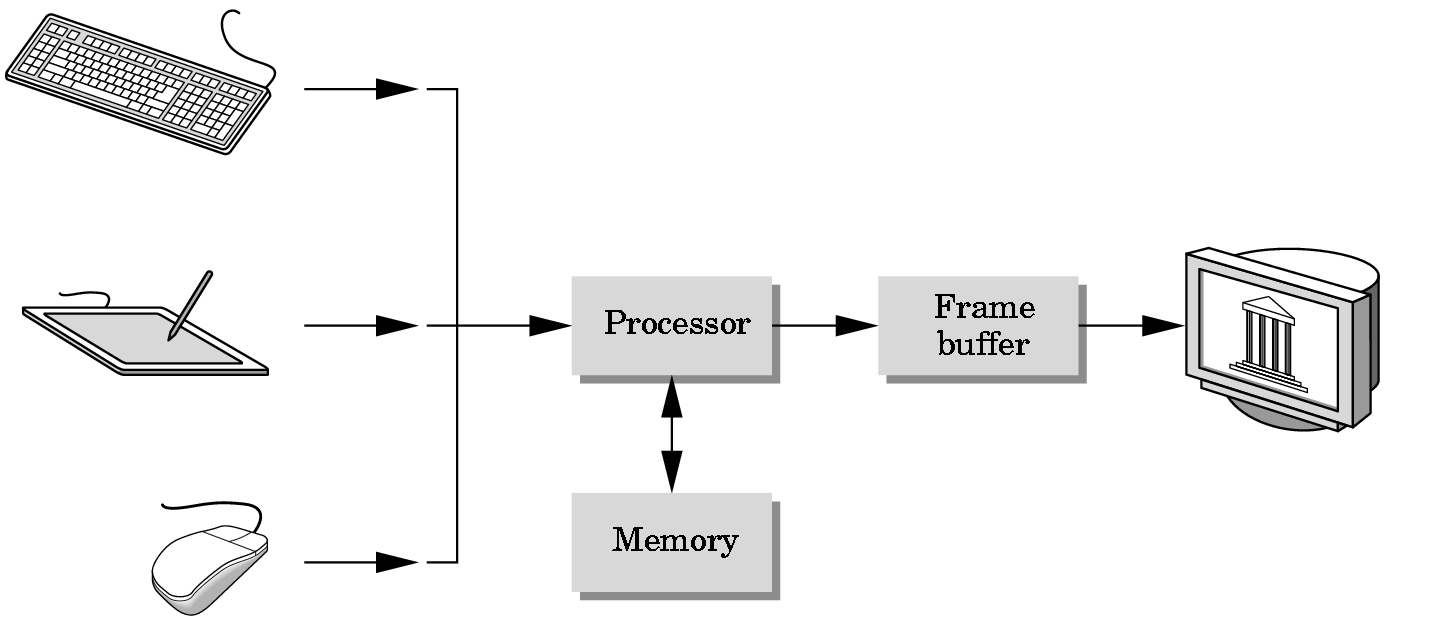
\includegraphics[scale=0.2]{img.png}
		\end{figure}
		\begin{center}
			\begin{tikzpicture}[>=latex, scale=.6]
			\draw (3,-3) -- (4,-2) -- (4,0) -- (2,0) -- (1,-1) ;
			\draw (3,-1) -- (4,0);
			\draw  (1,-1) rectangle (3,-3);
			\node [below] at (2,-3.5) {model};
			\draw[->] (4.5,-2) -- node[above, align=center] {graphics\\software} (6.5,-2);
			\foreach \i in {0.0, -0.5,..., -3}{
				\draw[fill=black] (7.5, \i) rectangle (7.1, \i-0.4);
				\foreach \x in {7.5,8,...,10.5}{
					\draw (\x, \i) rectangle (\x-0.4, \i-0.4);
					\draw[fill=black] (\x, -2) rectangle (\x-0.4, -2.4);
				}
			}
			
			
			\node [below] at (9,-3.5) {frame buffer};
			\draw[->] (11,-2) -- node[above, align=center] {graphics\\hardware} (13,-2);
			\draw (14,0) rectangle (18,-3) ;
			\node [below] at (16,-3.5) {monitor screen};
			\draw (18, -3) -- (19, -2) -- (19, 1) -- (15, 1) -- (14, 0);
			\draw (18,0) -- (19,1);
			\draw[fill=black] (14.5,-0.5) rectangle (17.5,-2.5);
			\draw[fill=white] (16.5,-2.5) -- (17,-2) -- (17,-1) -- (16,-1) -- (15.5,-1.5);
			\draw[fill=white] (15.5,-1.5) rectangle (16.5,-2.5);
			\draw (17,-1) -- (16.5,-1.5);
			
		\end{tikzpicture}
		\end{center}
		
		\noindent
		Le immagini raster sono \textbf{matrici} che contengono valori che rappresentano il colore
		nella casella corrispondente agli indici con valori discretizzati.
		
		\noindent
		Di solito ci sono componenti di colore: i monitor generano il colore
		con sovrapposizione di luce rossa, verde e blu (Perché?)
		
		\noindent
		Caratteristiche principali (non le uniche): 
		\begin{itemize}
			\item \textbf{risoluzione} (dimensioni della matrice di pixel)
			\item \textbf{profondità di colore} (bit di memoria per pixel).
		\end{itemize}
		8-bit significano 256 colori, mentre 24-bit (o truecolor)
		rappresentano all’incirca 32 milioni di colori
		
		\noindent
		\textbf{Nota}: è la rappresentazione di uscita tipica di quasi tutti i
		display odierni, ma non è ovviamente l'unica possibile
		\begin{itemize}
			\item Es.: display vettoriali: riproducono disegni
			\item Il formato digitale creato internamente deve ovviamente
			corrispondere alla capacità del display scelto di riprodurlo
		\end{itemize}
		
		Nel processo di rasterizzazione delle immagini vettoriali la qualità della
		conversione dipende	dalla risoluzione dell'immagine originale (numero di punti o punti per pollice).
		
		\noindent
		Un effetto possibile può essere la scalettatura: effetto dell'\textbf{aliasing} delle alte frequenze.
		Si può ridurre tale effetto sfumando la luminosità e facendo quindi \textit{antialiasing}.
		
		\begin{figure}[h!]
			\centering
			
\includegraphics[scale=0.2]{alias.png}
			\hspace*{0.4cm}
			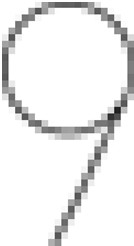
\includegraphics[scale=0.2]{alias1.png}
			\hspace*{0.4cm}
			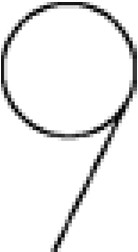
\includegraphics[scale=0.2]{alias2.png}
			\hspace*{0.4cm}
			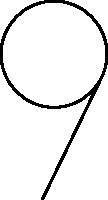
\includegraphics[scale=0.25]{alias3.png}
		\end{figure}
		
	\subsection{Aliasing}
		L'aliasing accade perché l'immagine è il campionamento di un segnale "continuo" che rappresenterebbe il dato misurabile.
		\[
			I(i, j) = I(i\Delta x, j\Delta y) = \iint F (x, y)\delta (x - i\Delta x)\delta (y - i\Delta y)
		\]
		
		\begin{center}
			\begin{tikzpicture}[>=latex, scale=0.5]
			\foreach \x in {0, 1, ..., 5}{
				\foreach \i in {0, -1, ..., -5}{
					\fill (\x,\i) circle (4pt);
				}
			}
			\draw[<->] (-0.5,-5) -- node[left] {$ \Delta y$} (-0.5,-4);
			\draw[<->] (0,-5.5) -- node[below] {$ \Delta x$} (1,-5.5);
		\end{tikzpicture}
		\end{center}
		
		Per il \textit{teorema di Shannon/Nyqvist} del campionamento, non si
		può ricostruire esattamente il segnale originale se la frequenza
		del segnale è superiore alla metà della frequenza di
		campionamento.
		
		\[
			v_{cx} = \dfrac{1}{\delta x} \geq 2v_{x max} \qquad 
			v_{cy} = \dfrac{1}{\delta y} \geq 2v_{y max} 
		\]
		
		Dove ci sono discontinuità del colore, ci sono componenti a
		frequenza alta, si creano artefatti. I filtri che fanno antialiasing attenuano le alte frequenze.
		
		
	\subsection{Caratteristiche Immagini raster}
		Le principali caratteristiche delle immagini raster sono:
		\begin{itemize}
			\item \underline{Risoluzione} (numero di righe e colonne matrice)
			\item \underline{Range dinamico}: rapporto tra minima differenza misurabile o
			rappresentabile e range di variabilità del segnale (luminosità). Corrisponde al numero di bit con cui codifichiamo il valore. Tipicamente 8 bit ma si può andare oltre:
			\begin{itemize}
				\item Immagini HDR
				\item Immagini mediche
				\item Dato che l'occhio umano non distingue così tante sfumature, lo
				scopo è di poter creare da esse rendering diversi che possano dare
				differenti effetti o informazioni
			\end{itemize}
			Il valore codificato dovrebbe corrispondere alla luminosità del
			punto generata dal monitor o acquisita dal sensore, ma la cosa
			è un po' più complicata a causa della \textbf{non-linearità della
			percezione umana}.
		\end{itemize}
		Insomma quello che c'è nel file non è quello che vediamo. Il rendering ed il dispositivo determinano la visualizzazione. E poi c'è il fattore legato alla percezione umana. 
		Ad esempio: immagini ad alto range dinamico (HDR) (Mantiuk et al 2005)
		
		\noindent
		La percezione umana amplifica le differenze del range dinamico ai bassi livelli. Macchine fotografiche e monitor applicano correzioni (gamma correction)
		
		\subsubsection{Colore}
			Le immagini raster da inviare ai display sono in genere a colori,
			per simulare il modo in cui vediamo il mondo (a colori).
			La rappresentazione del colore è generalmente una \textit{terna di
			valori RGB}.
			Per la riproduzione corrispondono alle intensità emesse da tre
			emettitori di luce a tre frequenze determinate (rosso, verde,
			blu) che danno origine in corrispondenza a un certo colore
			percepito dall'utente.
			
			\noindent
			\textit{Ma cosa significa questo?}
			
			\noindent
			Nei monitor si generano i colori nei punti della griglia per
			sintesi additiva: si mescolano due o più fasci luminosi di
			diversa.
			
			\noindent
			Nella stampa per sintesi sottrattiva: Due o più inchiostri
			sovrapposti assorbono diverse frequenze e cambiano la luce
			diretta all'occhio.
			
			\noindent
			Non tutti i colori possono essere generati in mescolanza
			additiva o sottrattiva di tre colori primari
			La scelta di \textbf{Rosso Verde Blu} come \textit{primari additivi} e \textbf{Giallo,
			Magenta e Cyan (e nero)} \textit{sottrattivi} cerca di massimizzare i
			colori rappresentabili
		
			\begin{wrapfloat}{figure}{I}{0pt}
				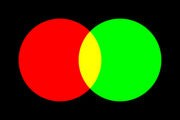
\includegraphics[width=0.3\textwidth]{colors}
			\end{wrapfloat}
		
			\noindent
			L'uso delle 3 componenti di colore RGB è
			convenzionale e deriva dalla fisiologia della
			visione, che mostra che con 3 colori base si
			possono approssimativamente riprodurre i
			colori del mondo reale.
			
			\noindent
			I colori visibili però derivano invece da una
			variazione continua di lunghezza d'onda delle
			radiazioni elettromagnetiche in un intervallo
			percettibile di valori circa 370-730 nm.
			
			\noindent
			\textbf{Percezione del colore}: nella retina ci sono 3 tipi di coni, che
			hanno differenti sensitività a diverse frequenze S,M,L
			Possiamo fare il matching delle frequenze con la risposta dei
			recettori.
			
			\bigskip
			
			Il "colore" percepito è dato da 3 grandezze scalari, funzione
			dello spettro della luce incidente.
			La corrispondenza non è iniettiva. Spettri diversi possono
			corrispondere allo stesso colore percepito: metamerismo
			Conseguenza: Per riprodurre un colore, non è necessario
			riprodurre lo spettro. È sufficiente che le risposte L, M, S dei
			coni siano uguali.
			Può cambiare in funzione dell'illuminazione.
			
			\noindent
			\textbf{Metamerismo}: consiste nella possibilità di ottenere un effetto ottico tale che l'occhio percepisca la stessa sensazione di colore in presenza di luce con distribuzione spettrale diversa dal colore puro in questione.
			Si tratta di un'illusione ottica basata sulla natura dell'interpretazione del colore da parte dell'occhio umano, è possibile creare la sensazione di un colore "puro", formato, selezionando la sola lunghezza d'onda che genera quella determinata sensazione di colore miscelando a dovere più lunghezze d'onda differenti, un esempio è il bianco di una lampada fluorescente formato da spettri non uniformi, in questo caso la temperatura di colore che si trova sulle confezioni è la temperatura a cui deve essere un corpo nero perché l'occhio umano percepisca la stessa sensazione di colore.
			Il fenomeno si ha quando colori che appaiono all'occhio identici sotto una certa luce, mostrano tonalità differenti se illuminati con una luce diversa. In sostanza c'è metamerismo quando due colori si equivalgono sotto una fonte di luce, ma risultano differenti ad altre esposizioni.
			
		\subsubsection{Legge di Grassman}
			L'uomo è in grado di fare match di colori mischiando 3 (o
			più) colori detti primari. Se la luce test $ T $ ha un certo colore:
			\[
				T = aP1 + bP2 + cP3
			\]
			il match si verifica lineare.
			
		\subsubsection{Funzioni di Matching}
			Data una terna di colori di base possiamo studiare il matching
			dei colori sugli osservatori in funzione della frequenza.
			Componenti colore CIERGB ricavate dall'integrale delle
			frequenze dello stimolo su tutto il range.
			
			\begin{align*}
				L &= \int \Phi (\lambda) L (\lambda) \diff\lambda \\
				M &= \int \Phi (\lambda) M (\lambda) \diff\lambda \\
				S &= \int \Phi (\lambda) S (\lambda) \diff\lambda 				
			\end{align*}
			
			Rappresentazione con matrice:
			\[
			C =
			\begin{pmatrix}
			\overline{r} (\lambda_1) & \dots & \overline{r}(\lambda_N) \\
			\overline{g} (\lambda_1) & \dots & \overline{g}(\lambda_N) \\
			\overline{b} (\lambda_1) & \dots & \overline{b}(\lambda_N) 
			\end{pmatrix}
			\]
			\[
			\Phi =
			\begin{pmatrix}
			\phi(\lambda_1)\\
			\vdots \\
			\phi (\lambda_N) 
			\end{pmatrix}
			\]
			
	\section{Schema di un'applicazione grafica}
		Vi è una descrizione di qualche tipo (procedurale o meno) del
		mondo che deve essere rappresentato. La produzione di tale
		descrizione (modello) prende il nome di \textbf{modellazione}.
		
		\noindent
		Da tale descrizione si ottiene una immagine visualizzabile da
		un display tale processo è chiamato globalmente \textbf{rendering}.
		
		\noindent
		La sequenza di procedure ed algoritmi che implementano il
		rendering prende il nome di \textbf{pipeline grafica}.
		
		\noindent
		Se l'applicazione è interattiva, il disegno dev'essere riprodotto
		in real time mentre l'utente interagisce con la scena mediante
		dei dispositivi.
			
	\subsection{Modello della scena}
		Nelle applicazioni 2D può essere un disegno da riprodurre sul
		display a meno di una trasformazione geometrica e mappatura
		sui pixel.
		Nelle applicazioni 3D di cui ci interesseremo sarà invece un
		vero e proprio modello del "mondo" che vogliamo vedere (e
		con cui vogliamo interagire) e l'immagine sarà generata
		simulando il processo di acquisizione di immagini di una
		telecamera "virtuale".
		
		\noindent
		Dati gli oggetti della scena, quindi dovremo "simulare" la geometria
		e la fisica della formazione delle immagini (luce, colore)
		
	\subsection{Rendering della scena}
		Il passaggio dalla rappresentazione all'immagine si definisce
		\textit{rendering}.
		
		\noindent
		Comprende tutti gli algoritmi per creare l'immagine per il
		display, che supporremo voglia un'immagine raster.
		
		\noindent
		Quindi se partiamo da una \textbf{rappresentazione 2D} (grafica
		vettoriale) il rendering consiste in:
		\begin{enumerate}
			\item Trasformazione delle primitive in rappresentazioni di colore sui pixel
			(rasterizzazione)
			\item Eventuale modifica interattiva del disegno
		\end{enumerate}
		Se partiamo da una \textbf{rappresentazione di scena 3D} il rendering consiste in:
		\begin{enumerate}
			\item Proiezione della scena sul piano immagine della telecamera virtuale
			\item Trasformazione della scena proiettata in rappresentazioni di colore
			sui pixel (rasterizzazione)
			\item Eventuale interazione con la scena e conseguenteupdate del
			rendering
		\end{enumerate}
		
		Il rendering comprende molti calcoli da svolgere, la \textbf{complessità} dipende dall'applicazione di interesse:
		\begin{itemize}
			\item Applicazioni interattive, real-time:
			\begin{itemize}
				\item Frame rate alto (>10 fps)
				\item Tempo di rendering del singolo frame prefissato
				\item Si può/deve sacrificare la qualità per garantire l’interattività
			\end{itemize}
			\item Applicazioni non interattive (computer animation, grafica
			pubblicitaria)
			\begin{itemize}
				\item l'obiettivo primario: massima qualità delle immagini di sintesi
				\item Non si hanno vincoli sul tempo di generazione del singolo frame
				\item Animazioni calcolate frame by frame da PC cluster, ricomposte
				successivamente nella successione temporale corretta
			\end{itemize}
		\end{itemize}
		
		Come si implementa la fase di rendering?
		\begin{itemize}
			\item Applicazioni interattive: si avvalgono pesantemente delle moderne schede grafiche (HW
				dedicato al processing di dati 3D)
			\item Applicazioni non interattive: fanno uso di ambienti di rendering più sofisticati e flessibili (ad es. RenderMan), spesso eseguiti SW su cluster di PC
		\end{itemize}
		
	\section{Modellare lo spazio}
		Richiamiamo le nozioni basilari di geometria per modellare lo
		spazio e gli oggetti:
		\begin{itemize}
			\item \textbf{Scalari}: unidimensionali, possono rappresentare grandezze fisiche
			con numeri
			\item \textbf{Punti}: rappresentano una posizione nello spazio
			\item \textbf{Vettori}: rappresentano le direzioni o le distanze tra punti in 2D o 3D
		\end{itemize}
		Per definire una posizione nello spazio dobbiamo introdurre un
		sistema di riferimento con un punto fisso detto origine e una
		terna di direzioni ortogonali
		
		\subsection{Scalari}
			Gli scalari S costituiscono un corpo (tipicamente useremo IR)
			con due operazioni, somma e moltiplicazione, che soddisfano
			le seguenti relazioni:
			
			\begin{multicols}{2}
				\begin{center}
					$ \forall \alpha,\beta,\gamma \in S $
				
				\noindent
				\textbf{Commutatività}
				\begin{align*}
					\alpha + \beta &= \beta + \alpha \\
					\alpha \beta &= \beta\alpha
				\end{align*}
				
				\textbf{Associatività}
				\begin{align*}
					\alpha + (\beta + \gamma) &= (\beta + \alpha) + \gamma \\
					(\alpha\beta)\gamma &= \alpha(\beta\gamma)
 				\end{align*}
				
				\textbf{Distribuzione}
				\[
					\alpha(\beta + \gamma) = \alpha\beta + \alpha\gamma
				\]
				
				\columnbreak
				
				\textbf{Elementi neutri}
				\begin{align*}
					\exists 0 \in S \: &: \: \forall \alpha \in S \quad \alpha + 0 = \alpha \\
					\exists 1 \in S \: &: \: \forall \alpha \in S \quad \alpha 1 = \alpha 
				\end{align*}
				
				\textbf{Elementi inversi}
				\begin{align*}
				\forall \alpha \in S \quad & \exists (-\alpha) \in S \: : \: \alpha + 0 = \alpha \\
				\forall \alpha \in S \quad & \exists \alpha^{-1} \in S \: : \: \alpha\alpha^{-1} = 1 
				\end{align*}
				\end{center}
			\end{multicols}
			
		\subsection{Vettori}
			I vettori costituiscono un \textbf{gruppo
			abeliano} (commutativo) $ V $ in cui e
			definito il \textbf{prodotto di un vettore
			per uno scalare}.
		
			\begin{multicols}{3}
				\begin{center}
				\textbf{Chiusura}
				\begin{align*}
					\vec{u} + \vec{v} \in V &\quad \forall \vec{u}\vec{v} \in V \\
					\alpha \vec{v} \in V &\quad \forall \alpha \in S \: \vec{v} \in V
				\end{align*}
				\columnbreak
				
				\textbf{Proprietà Algebriche}
				\begin{align*}
					\vec{u} + \vec{v} &= \vec{v} + \vec{u} \\
					\vec{u} + (\vec{v} + \vec{w}) &=  (\vec{u} + \vec{v}) + \vec{w} \\
					\alpha(\vec{u} + \vec{v}) &= \alpha\vec{u} + \alpha\vec{v} \\
					(\alpha + \beta)\vec{u} &= \alpha\vec{u} + \beta\vec{u}
				\end{align*}
				
				\begin{align*}
					\exists 0 &\in V \: : \: \forall \vec{u} \in V \quad \vec{u} + 0 = \vec{u} \\
					\forall \vec{u} &\in V \: \: \exists(-\vec{u}) \in V \: : \: \vec{u} + (-\vec{u}) = \vec{0}
				\end{align*}
			\end{center}
			\end{multicols}
		
			La definizione è totalmente
			astratta, ma per semplicità
			conviene considerare due utili
			esempi di spazi vettoriali lineari: Geometrico e Algebrico.
			
			\noindent
			Un esempio concreto e dato
			dai segmenti orientati liberi,
			ovvero senza un punto di
			applicazione specificato
			Il prodotto con uno scalare
			(numeri reali) cambia la
			lunghezza del vettore.
			La somma di due vettori e
			data dalla regola del
			parallelogramma.
			
			\begin{tikzpicture}[>=latex, baseline=0.5cm]
				\draw[thick, ->] (0,-2) -- (2,0) node[midway, left] {$ \vec{v} $};
				\draw[thick, ->] (0,-3) -- (3,0) node[midway, left] {$ 2\vec{v} $};
			\end{tikzpicture}
			\hspace*{0.5cm}
			\begin{tikzpicture}[>=latex, baseline=0.5cm]
				\draw[thick, <-] (0,-2) -- (2,0) node[midway, left] {$ -\vec{v} $};
				\draw[thick, ->] (4,-2) -- (6,0) node[midway, left] {$ \vec{v} + \vec{u} $};
				\draw[thick, ->] (4,-2) -- (5.5,-1.5) node[midway, below] {$ \vec{v}$};
				\draw[thick, ->] (5.5,-1.5) -- (6,0) node[midway, right] {$ \vec{u} $};
			\end{tikzpicture}
			
			\vspace*{0.5cm}
			
			\noindent
			Un altro esempio è dato dall'insieme delle n-ple ordinate di $ \R^n $.
			\[
				\vec{v} = (\beta_1, \dots, \beta_n) \quad \beta_i \in \R \forall i
			\]
			Il prodotto per uno scalare e la somma di due vettori sono
			definiti in modo del tutto naturale:
			\begin{align*}
				(\alpha_1, \dots, \alpha_n) + (\beta_1, \dots, \beta_n) &= 
				(\alpha_1 + \beta_1, \dots, \alpha_n + \beta_n) \\
				\alpha(\beta_1, \dots, \beta_n) &= (\alpha\beta_1, \dots, \alpha\beta_n)
			\end{align*}
			E' facile vedere qual è l'elemento neutro e qual è l'inverso di un
			vettore.
			
		\subsubsection{Indipendenza lineare}
			Dati n vettori non nulli, si dicono \textbf{linearmente indipendenti} se
			qualsiasi loro combinazione lineare a coefficienti non tutti nulli
			è diversa dal vettore nullo.
			\[
				\alpha_1\vec{v}_1 + \dots + \alpha_n \vec{v}_n = \vec{0} \: \Leftrightarrow \: \alpha_i = 0 \forall i
			\]
			Si dice \textbf{dimensione} di uno spazio vettoriale il massimo numero
			di vettori linearmente indipendenti.
			
			\noindent
			In uno spazio vettoriale a dimensione n, un insieme di n vettori
			linearmente indipendenti si dice una \textbf{base} per lo spazio.
			Ogni vettore può essere scritto come combinazione lineare dei
			vettori di una base.
		\subsubsection{Rappresentazione in componenti}
			Fissata quindi una \textbf{base in uno spazio vettoriale}, ad ogni
			vettore corrisponde una n-pla di scalari, ovvero i coefficienti
			dello sviluppo lineare del vettore nei vettori di base; tali scalari
			sono le componenti del vettore rispetto alla base data.
			
			\noindent
			In genere il corpo è dato dai reali; abbiamo quindi ottenuto la
			rappresentazione concreta vista prima di uno spazio vettoriale
			astratto come insieme di n-ple di $ \R^n $.
			Tale rappresentazione dipende dalla base scelta.
			
		\subsection{Punti}
			I vettori non rappresentano punti nello spazio, ma solo
			spostamenti. Per poter introdurre il concetto di \textbf{posizione} si
			deve passare agli \textbf{spazi affini} che sono degli spazi vettoriali a
			cui si aggiunge il concetto astratto di punto.
			
			\noindent
			I punti sono definiti in senso astratto come nuovi elementi con
			cui e possibile effettuare solo una operazione: la sottrazione
			tra punti.
			
			
			La differenza di due punti è un vettore: $ P - Q = \vec{v} $
			
			Dato un punto $ Q $ ed un vettore $ \vec{v} $, esiste un unico punto $ P $
			tale che $ P - Q = \vec{v} $.
			
			Si definisce quindi una somma tra un punto ed un vettore il
			cui risultato e un punto: $ P = Q + \vec{v} $
			
			\noindent
			\textit{Attenzione}: non ho sommato Q da entrambe le parti
			dell'equazione precedente.
			
			\noindent
			L'interpretazione geometrica è immediata; i punti sono
			locazioni nello spazio e la differenza di due punti e data dal
			vettore che li congiunge; è importante non confondere punti e
			vettori, sono entità geometriche ben distinte.
			
		\subsection{Combinazioni affini}
			Non è definita una somma tra punti e neppure un prodotto di
			uno scalare per un punto; in generale sono operazioni non
			lecite, ma c'è una eccezione.
			
			\noindent
			Si prendano tre punti P, Q ed O e si consideri il seguente
			punto: 
			\[
				P' = \alpha(P - O) + \beta(Q - O) + O 
			\]
			$ P' $ non dipende da $ O $, ma solo dai punti $ P $ e $ Q $, se e solo se $ \alpha + \beta = 1 $
			
			\noindent
			In questo caso $ P' $ è la \textbf{combinazione affine} di $ P $ e $ Q $, e si scrive,
			a volte in modo improprio, come \textbf{somma pesata dei punti}.
			
			\noindent
			\textit{La combinazione affine di due punti distinti descrive la retta
			passante per i due punti}.

			\noindent
			La combinazione affine si estende in modo naturale a $ n $ punti.
			\[
				P' = \sum_{i} \alpha_i P_i , \quad \sum_{i} \alpha_i = 1 \: \: \alpha_i \in \R
			\]
			Un insieme di punti si dice \textbf{affinemente indipendente} se
			\textit{nessun punto è combinazione affine degli altri}.
			
		\subsubsection{Combinazione Convessa}
			La combinazione convessa è una combinazione affine con pesi
			positivi.
			
			\noindent
			Nel caso della combinazione convessa di due
			punti, il punto risultante giace sul segmento
			che congiunge i due punti. Se i pesi sono
			entrambi pari a $ 0.5 $, il punto risultante si trova
			a metà tra i due.
			
			\begin{tikzpicture}[scale=0.7,baseline=0.5cm]
				\draw (0,-2) -- (2,0);
				\fill (0,-2) circle (2pt) coordinate [label=below:$P$] (a)
					  (2,0) circle (2pt) coordinate [label=above:$Q$] (b)
					  (1,-1) circle (2pt) coordinate [label=left:$\dfrac{P+Q}{2}$] (c);
			\end{tikzpicture}
			\hspace*{2.5cm}
			\begin{tikzpicture}[scale=0.7,baseline=0.5cm]
				\draw (0,-2) -- (1,0) -- (4,-2) -- cycle;
				\fill (0,-2) circle (2pt) coordinate [label=below:$P$] (a)
					(1,0) circle (2pt) coordinate [label=above:$Q$] (b)
					(4,-2) circle (2pt) coordinate [label=above:$R$] (c)
					(1.7,-1.3) circle (2pt) coordinate [label=left:$\dfrac{P+Q+R}{3}$] (d);
			\end{tikzpicture}
			
			\noindent
			Nel caso di $ n $ punti che formano un poligono
			convesso, il punto risultante si trova all'interno del poligono.
			Se tutti i pesi sono uguali a $ 1/n $, il punto risultante si chiama
			\textbf{centroide} dell'insieme dei punti.
			
		\subsubsection{Guscio Convesso}
			Un insieme $ C \in \R^n $ è convesso se per ogni coppia di punti $ P_1, P_2 \in C$ 
			si ha che $ P' = \alpha(P_1 - P_2 ) + P_2 $ appartiene
			a $ C $ per ogni $ \alpha \in [0, 1] $  ovvero tutti i punti sul segmento che
			unisce $ P_1 $ con $ P_2 $ appartengono all'insieme $ C $.
			
			\noindent
			Il guscio convesso (\textit{convex hull}) di un insieme di punti è la più
			piccola regione convessa che contiene tutti i punti dati.
			
		\subsection{Prodotto interno}
			In uno spazio affine non è ancora definito il concetto di
			distanza o di angolo tra vettori; questi si ottengono passando ad
			uno spazio euclideo che è uno spazio affine provvisto di
			un \textbf{prodotto interno tra vettori (\textit{prodotto scalare})} che è definito come:
			
			Dati due vettori $ a = [a_i]_1^n $ e $ b = [b_i]_1^n $ di $ \R^n $
			\[
				\sum_{1}^{n} a_i b_i = 
				\begin{bmatrix}
					a_1 & \dots & a_n
				\end{bmatrix}
				\begin{bmatrix}
					b_1 \\
					\vdots \\
					b_n
				\end{bmatrix}
				= a'b
			\]
			
			
			che soddisfa le seguenti relazioni:
			\begin{align*}
				\vec{u} \cdot \vec{v} &= \vec{v}\cdot \vec{u} \in S \\
				(\alpha\vec{u} + \beta\vec{v}) \cdot\vec{w} &= 
				\alpha\vec{u}\cdot\vec{w} + \beta\vec{v}\cdot\vec{w} \\
				\vec{v}\cdot\vec{v} > 0 & \: \: (\vec{v} \neq \vec{0}) \\
				\vec{0}\cdot\vec{0} &= 0
			\end{align*}
			
			Se il prodotto interno di due vettori è nullo, diremo che i \textbf{due
			vettori sono ortogonali}. 
			Grazie al prodotto interno e possibile definire la \textbf{lunghezza di
			un vettore} (e quindi la distanza tra due punti) e l'\textbf{angolo} tra
			due vettori.
			
			\noindent
			\textbf{Norma di un vettore}:
			\[
				\lVert \vec{v} \rVert = \sqrt{\vec{v}\cdot\vec{v}} \quad 
				\cos \theta = \dfrac{\vec{v}\cdot\vec{u}}{\lVert \vec{v} \rVert \: \lVert \vec{u} \rVert}
			\]
			
			Il prodotto scalare può essere usato, ad esempio, per trovare la
			proiezione di un vettore lungo una retta.
			Sia dato il vettore $ \vec{v} $ e la retta con direzione identificata dal
			vettore di lunghezza unitaria $ u $; il vettore ottenuto proiettando
			v lungo la retta sarà della forma $ \vec{v}' = t\vec{u} $ dove $ t $ è un parametro,
			si può dimostrare che $ t = \vec{v} \cdot \vec{u} $
			
			\begin{center}
				\begin{tikzpicture}[>=latex]
				\draw (0,-2) -- (5,-2);
				\draw[ultra thick, ->] (1,-2) -- (2,-2) node[above] {$ \vec{u} $};
				\draw[ultra thick, ->] (1,-2) -- (4,-2) node[below] {$ (\vec{v}\cdot\vec{u})\vec{u} $};
				\draw[->] (1,-2) -- (4,0) node[outer sep=4pt,left] {$ \vec{v} $};
				\draw[dashed] (4,0) -- (4,-2);
			\end{tikzpicture}
			\end{center}
			
		\subsection{Normalizzazione}
			Un vettore è normalizzato se la sua lunghezza è $ 1 $; dato un
			vettore qualsiasi lo si può normalizzare moltiplicandolo per il
			reciproco della sua lunghezza.
			
			\noindent
			\textit{Un vettore normalizzato si dice anche \textbf{versore}}
			
			Una base è \textbf{ortonormale} se e formata da versori a due a due
			ortogonali:
			\[
				(e_1, \dots, e_n) \: : \: \lVert e_i \rVert = 1 \: \forall i \quad \textup{e}
				\quad e_i\cdot e_j = 0 \quad \forall i \neq j
			\]
			Data una base ortonormale il prodotto interno tra due vettori
			si esprime come somma dei prodotti delle componenti (usuale
			prodotto scalare di vettori)
			\[
				\vec{v} \vec{w} = v_1 w_1 + \dots + v_n w_n
			\]
			data una base qualsiasi è sempre possibile derivare da essa una base
			ortonormale (procedimento di \textit{Gram-Schmidt})
			
		\subsection{Terne}
			In tre dimensioni una base ortonormale si dice \textbf{destrorsa}, se la
			rotazione attorno ad $ \vec{e}_3 $ che porta $ \vec{e}_1 $ a coincidere con $ \vec{e}_2 $ è
			antioraria se vista dalla parte positiva di $ \vec{e}_3 $ .
			Se tale rotazione è oraria allora la base è \textbf{sinistrorsa}.
			
			\noindent
			Si può usare la \textit{prima regola della mano destra}: se si pone il
			pollice nella direzione di $ \vec{e}_3 $ , la rotazione che porta $ \vec{e}_1 $ in $ \vec{e}_2 $ deve seguire il modo naturale con cui si piegano le altre dita.
			
			\noindent
			Oppure la \textit{seconda regola della mano destra} per determinare la
			destrorsità: se si riesce a porre i tre vettori di base in
			corrispondenza con pollice, indice e medio della mano destra,
			tenuti perpendicolari l'uno all'altro, la base e destrorsa.
			La scelta di un orientamento è del tutto arbitraria, basta
			essere coerenti. Di norma si usano basi destrorse.
			
		\subsection{Sistemi di riferimento (frame)}
			Il concetto di base si estende a quello di riferimento in uno
			spazio affine (o euclideo) specificando, oltre alla base, anche
			un punto $ O $ detto origine del riferimento.
			
			\noindent
			Poiché ogni vettore è sviluppabile in una base data ed ogni
			punto esprimibile come somma di un punto dato e di un
			vettore, dato un riferimento $ (\vec{e}_1, \vec{e}_2, \vec{e}_3, O) $, i punti ed i vettori
			dello spazio saranno esprimibili nel seguente modo:
			\begin{align*}
				\vec{v} &= v_1\vec{e}_1 + v_2\vec{e}_2 + v_3\vec{e}_3 \\
				P &= p_1\vec{e}_1 + p_2\vec{e}_2 + p_3\vec{e}_3 + O
			\end{align*}
			Un riferimento \textbf{cartesiano} è dato da un riferimento la cui base
			di vettori sia ortonormale. 
			
			\noindent
			Un riferimento è destrorso se lo è la sua base.
			
		\subsection{Coordinate omogenee}
			Definiamo il prodotto di un punto per 1 e per 0: $ \quad P\cdot 1 = P \quad P\cdot 0 = 0 $.
			
			In questo modo possiamo definire le coordinate omogenee di
			un punto e di un vettore rispetto al riferimento $ (\vec{e}_1 , \vec{e}_2 , \vec{e}_3 ,O) $.
			\begin{align*}
				\vec{v} &= (v_1, v_2, v_3, 0) \\
				P &= (p_1, p_2, p_3, 1)
			\end{align*}
			La scelta di 0 e 1 come ultima coordinata per vettori e punti è
			arbitraria, andrebbe bene qualsiasi valore:
			
			\noindent
			Tale scelta però permette il \textbf{type checking}: si trattano le 4-ple delle
			coordinate omogenee come vettori quando si effettua una qualsiasi
			combinazione lineare di punti e vettori, usando le usuali regole, se
			l'ultima coordinata del risultato è 0, allora il risultato è un vettore;
			se è pari a 1 allora il risultato è un punto!
			
			\noindent
			Se non è ne 0 ne 1, allora si è effettuata una operazione non lecita
		
		\subsection{Riepilogo}
		
		\begin{itemize}
			\item Gli scalari sono numeri reali
			\item I vettori identificano direzioni nello spazio
			\item I punti determinano posizioni nello spazio
			\item Operazioni ammesse:
			somma e prodotto tra scalari, prodotto di scalari per vettori, somma
			di vettori, differenza di punti, somma di un punto con un un vettore,
			combinazioni affini.
			\item Il prodotto scalare permette di determinare la lunghezza dei
			vettori, la distanza tra punti e l'angolo tra due vettori
			\item Conviene lavorare in una base ortonormale; in questo caso il
			prodotto scalare tra due vettori e particolarmente semplice
			\item I tre assi che formano la base si chiamano assi coordinati e si
			indicano con $ x, y $ e $ z $ (a volte useremo anche 1, 2 e 3).
		\end{itemize}
		
		\subsection{Prodotto vettore}
		Nel caso particolare delle tre dimensioni è utile introdurre
		un'ulteriore operazione tra vettori: \textbf{il prodotto vettore}.
		
		\noindent
		Si tratta di un caso particolare di prodotto denominato
		\textbf{esterno}; in tre dimensioni particolarmente semplice:
		\[
		\vec{u}\times\vec{v} = (u_y v_z - u_y v_y,\: u_z v_x - u_x v_z,\: u_x v_y - u_y v_x)
		\]
		Si dimostra che il prodotto vettore di due vettori $ \vec{u} $ e $ \vec{v} $ è un
		vettore ortogonale al piano contenente i due vettori e di
		modulo pari all'area definita da $ \vec{u} $ e $ \vec{v} $. Il verso è scelto in modo
		tale che $ (\vec{u}, \vec{v}, \vec{u} \times \vec{v}) $ formino una terna destrorsa.
				
		\noindent
		\textit{Attenzione}: il prodotto vettore (a differenza delle proprietà affini
		dello spazio) dipende dalla scelta del tipo di base, destrorsa o sin.
				
		\textbf{Esempio:} Data una direzione espressa dal vettore unitario $ \vec{v} $, voglio
		creare un sistema di riferimento ortogonale con l'asse $ z $
		coincidente con $ \vec{v} $. Come faccio?
		\begin{itemize}
			\item Prendo un qualunque vettore $ \vec{a} $ non parallelo a $ \vec{v} $.
			\item Prendo la direzione dell'asse $ x $ $ \vec{e}_1 $ uguale a $ \vec{v} \times \vec{a} $.
			\item Prendo la direzione dell'asse $ y $ $ \vec{e}_2 $ uguale a $ \vec{v} \times \vec{e}_1 $.
		\end{itemize}
				
	\subsection{Matrici e trasformazioni}
		Una matrice è essenzialmente un array bidimensionale di
		elementi; per i nostri scopi gli elementi saranno sempre degli
		scalari, tipicamente numeri reali.
		
		Una matrice $ A $ puo essere moltiplicata per uno scalare $ \beta $
		ottenendo una matrice $ C = \beta A $ definita nel seguente modo:
		\[
			c_{i j} = \beta a_{i j} \quad \forall i, j
		\]
		
		Due matrici $ A $ e $ B $ si possono sommare se e solo se hanno lo
		stesso numero di righe e di colonne; in tal caso si ha $ C = A + B $ data da:
		\[
			c_{i j} = a_{i j} + b_{i j} \quad \forall i, j
		\]
		
		Il prodotto tra matrici e definito solo quando il numero di
		colonne della prima matrice è uguale al numero di righe della
		seconda. Se $ A $ è una matrice $ N\times M $ e $ B $ e una matrice $ M\times K $, allora
		si ha $ C = AB $ (di dimensioni $ N\times K $) data da:
		\[
			c_{i j} = \sum_{l = 1}^{M} a_{i l} b_{l j}
		\]
		Il prodotto tra matrici è \textbf{associativo} ($ (AB)C = A(BC) $), ma \textbf{non commutativo} (in generale $ AB\neq BA $)
			
	\subsection{Matrice trasposta}
		Indicata con il simbolo $ A_T $ , è la matrice ottenuta scambiando le
		righe con le colonne di $ A $: 
		\[
			a_{i j}^T = a_{j i} 
		\] 
		Quindi se $ A $ è $ N\times M $, allora la sua trasposta è $ M\times N $.
		
		\noindent
		Per i vettori trasporre equivale a trasformare un vettore riga in
		un vettore colonna e viceversa
		D'ora in poi quando parleremo di \textbf{trasformazione} di un vettore
		$ \vec{v} $ con una matrice $ A $ intenderemo sempre l'usuale \textit{prodotto di
		matrici} tra $ A $ e il trasposto di $ \vec{v} $ inteso come matrice con una
		sola colonna, es.:
		\[
			A\vec{v} =
			\begin{pmatrix}
				a_{1 1} & a_{1 2} \\
				a_{2 1} & a_{2 2}
			\end{pmatrix}
			\begin{pmatrix}
				v_1 \\
				v_2
			\end{pmatrix}
			=
			\begin{pmatrix}
				a_{1 1}v_1 + a_{1 2}v_2 \\
				a_{2 1}v_1 + a_{2 2}v_2
			\end{pmatrix}
		\]
		
	\subsection{Determinante}
		Importante parametro per le matrici quadrate, indicato con il
		simbolo $ det A $ o con il simbolo $ |A| $. Si definisce
		ricorsivamente:
		
		Il determinante di una matrice $ 2x2 $ è definito da:
		\[
			\begin{vmatrix}
				a_{1 1} & a_{1 2} \\
				a_{2 1} & a_{2 2}
			\end{vmatrix}
			= a_{1 1}a_{2 2} - a_{1 2}a_{2 1}
		\]
		Il determinante di una matrice $ N\times N $ è dato dalla formula:
		\[
			detA = \sum_{j = 1}^{N} (-1)^{j + k} a_{j k} detA_{j k}
		\]
		dove $ k $ e una colonna qualsiasi di $ A $ e dove il simbolo $ A_{j k} $ indica
		la matrice $ (N-1)\times(N-1) $ ottenuta da $ A $ eliminando la riga $ j $ e la
		colonna $ k $. Si può dimostrare che $ det(AB) = detA\: detB $
		
		\noindent
		Si può dimostrare che una matrice e invertibile se e solo se il suo
		determinante è diverso da 0; in tal caso si ha:
		\[
			a_{i j}^{-1} = (-1)^{i+j} \dfrac{\textup{det}A_{i j}}{\textup{det}A}
		\]
	\subsection{Matrici: trasformazioni e cambiamento di base}
		Abbiamo visto cosa significa applicare una matrice ad un vettore
		\begin{itemize}
			\item Le matrici quadrate rappresentano quindi delle\textbf{ applicazioni
			lineari} di uno spazio vettoriale in sé (formano un gruppo non
			abeliano).
			\item Tutte le applicazioni lineari di uno spazio vettoriale in sé sono
			esprimibili tramite \textbf{matrici quadrate}.
			\item L'applicazione di più di una matrice ad un vettore si effettua
			sfruttando l'algebra delle matrici; ad esempio applicare prima
			$ A $, poi $ B $ ed infine $ C $ equivale ad applicare la matrice $ CBA $.
		\end{itemize}
		Abbiamo detto che dato uno spazio vettoriale esistono infinite
		basi. Nella rappresentazione concreta il \textbf{cambiamento da una
		base ad un'altra} è descritto da una matrice.
	
		\noindent
		In generale dato un vettore $ (v_1 , v_2 , v_3 ) $, la sua trasformazione
		in $ (v'_1 , v'_2 , v'_3 ) $ tramite la matrice $ M $ puo essere vista come :
		\begin{itemize}
			\item Una trasformazione identificata da M del vettore fissata la base (\textbf{trasformazione attiva}).
			\item Un cambiamento di base indotto dalla matrice $ M^{-1} $ tenendo fisso il vettore (\textbf{trasformazione passiva}).
		\end{itemize}
		
	\subsection{Cambio di riferimento}
		L'idea si ripropone negli stessi termini per i sistemi di
		riferimento.\\
		Dati due riferimenti $ (\vec{e}_1 , \vec{e}_2 , \vec{e}_3 ,O) $ e 
		$ (\vec{e'}_1 ,\vec{e'}_2 ,\vec{e'}_3 ,O) $ si tratta
		di trovare una matrice $ 4\times 4 $ che permetta di ottenere le
		coordinate di un punto rispetto al secondo riferimento date le
		coordinate dello stesso punto rispetto al primo.
		
		Come nel caso dei cambiamenti di base di un riferimento, se $ T $
		è la trasformazione attiva che manda il primo riferimento nel
		secondo (e che manda le coordinate rispetto al secondo nelle
		coordinate rispetto al primo), allora $ T_{-1} $ e la matrice che
		trasforma le coordinate rispetto al primo riferimento nelle
		coordinate rispetto al secondo riferimento.
		
		\textbf{Esempio: }\\
		Determinare la rotazione che porta gli assi canonici 
		$ \vec{e}_1 =(1,0,0),\: \vec{e}_2 = (0,1,0),\: \vec{e}_3=(0,0,1) $
		in una qualunque terna 
		\begin{align*}
			\vec{e'}_1 &=(e'_{11} ,e'_{12} ,e'_{13} ), \\
			\vec{e'}_2 &=(e'_{21} ,e'_{22} ,e'_{23} ), \\
			\vec{e'}_3 &=(e'_{31} ,e'_{32} ,e'_{33} ) 
		\end{align*}
		La matrice di rotazione è data da:
		\[
			\begin{pmatrix}
				\vec{e}_1\vec{e'}_1 & \vec{e}_1\vec{e'}_2 & \vec{e}_1\vec{e'}_3 \\
				\vec{e}_2\vec{e'}_1 & \vec{e}_2\vec{e'}_2 & \vec{e}_2\vec{e'}_3 \\
				\vec{e}_3\vec{e'}_1 & \vec{e}_3\vec{e'}_2 & \vec{e}_3\vec{e'}_3 \\
			\end{pmatrix}
		\]
		
	\subsection{Traslazione}
	
		Una traslazione determinata dal vettore $ \vec{t} $ trasforma il punto $ P $ nel punto:
		\begin{wrapfloat}{figure}{O}{0pt}
			\begin{tikzpicture}[>=latex, scale=0.7]
			\draw[ultra thick, ->] (4,-3) -- (1,-4) node[above, left] {$ x $};
			\draw[ultra thick, ->] (4,-3) -- (7,-4) node[above, right] {$ y $};
			\draw[ultra thick, ->] (4,-3) -- (4,0) node[left] {$ z $};
			\draw[->] (3,-2) -- node[above] {$ \vec{t} $} (6,-1) node[right] {$ P + \vec{t} $};
			\fill (3,-2) circle (2pt) coordinate [label=below:$P$] (a);
			\end{tikzpicture}
		\end{wrapfloat}
		\[
			P' = P + \vec{t}
		\]
		
		In termini di componenti:
		\begin{align*}
			\vec{t} &= (t_x, t_y, t_z, 0) \\
			P &= (p_x, p_y, p_z, 1) \\
			P' &= (p_x + t_x,\: p_y + t_y,\: p_z + t_z,\; 1 )
		\end{align*}
		E' facile vedere che la matrice di
		trasformazione T t per le coordinate
		omogenee è:
		
		\[
			T_t =
			\begin{pmatrix}
				1 & 0 & 0 & t_x \\
				0 & 1 & 0 & t_y \\
				0 & 0 & 1 & t_z \\
				0 & 0 & 0 & 1 \\
			\end{pmatrix}
		\]
		
	\begin{wrapfigure}{r}{0.35\textwidth}
		\vspace{-30pt}
		\begin{tikzpicture}[>=latex, scale=0.7]
		\draw[ultra thick, ->] (4,-3) -- (1,-4) node[above, left] {$ x $};
		\draw[ultra thick, ->] (4,-3) -- (7,-4) node[above, right] {$ y $};
		\draw[ultra thick, ->] (4,-3) -- (4,0) node[left] {$ z $};
		\draw[->] (4,-3) -- (2,-5) node[left] {$ P $};
		\draw[->] (4,-3) -- (6,-5) node[right] {$ P' $};
		\draw[->, bend right] (3,-4) to (5,-4) ;
		\node at (4,-4) {$ \theta $};
		\end{tikzpicture}
		\vspace{-40pt}
	\end{wrapfigure}
	
	\subsection{Rotazione}
		Una rotazione di un angolo $ \theta $ in
		senso \textbf{antiorario} (prima regola della
		mano destra) \textbf{intorno all'asse} $ z $
		determina la seguente trasformazione
		di un punto $ P $ in $ P' $.
		
		\begin{align*}
			p'_x &= p_x\cos(\theta) - p_y \sin(\theta) \\
			p'_y &= p_x\sin(\theta) + p_y \cos(\theta) \\
			p'_z &= p_z			
		\end{align*}
		
		Si può facilmente dimostrare che per rotazioni intorno
		all'asse $ x $ e $ y $ si hanno le seguenti espressioni:
			\begin{align*}
				p'_y &= p_y \cos(\theta) - p_z \sin(\theta) \qquad &
					\qquad p'_z &= p_z \cos(\theta) - p_x \sin(\theta) \\
				p'_z &= p_y \sin(\theta) - p_z \cos(\theta) \qquad &
					\qquad p'_x &= p_z \sin(\theta) - p_x \cos(\theta) \\
				p'_x &= p_x \qquad & \qquad p'_y &= p_y
			\end{align*}

		\noindent
		\textbf{Matrici} che rappresentano le rotazioni rispetto agli assi coordinati:
		\[
			R_x(\theta) =
			\begin{pmatrix}
				1 & 0 & 0 & 0 \\
				0 & \cos\theta & -\sin\theta & 0 \\
				0 & \sin\theta & \cos\theta & 0 \\
				0 & 0 & 0 & 1
			\end{pmatrix}
			\quad
			R_y(\theta) =
			\begin{pmatrix}
			\cos\theta & 0 & \sin\theta & 0 \\
			0 & 1 & 0 & 0 \\
			-\sin\theta & 0 & \cos\theta & 0 \\
			0 & 0 & 0 & 1
			\end{pmatrix}
			\quad
			R_z(\theta) =
			\begin{pmatrix}
			\cos\theta & -\sin\theta & 0 & 0 \\
			\sin\theta & \cos\theta & 0 & 0 \\
			0 & 0 & 1 & 0 \\
			0 & 0 & 0 & 1
			\end{pmatrix}
		\]
		\textbf{Osservazioni:}\\
		Da notare che un \textit{vettore viene
		trasformato da una rotazione} (a
		differenza delle traslazioni che
		lasciano i vettori inalterati). \textit{Le matrici non commutano}.
		
		\noindent
		Le rotazioni rispetto agli assi cartesiani non commutano;
		provare a ruotare un oggetto di 90 gradi prima rispetto all'asse
		x e poi rispetto all'asse y. Ripetete quindi l'operazione prima
		rispetto all'asse y e poi rispetto all'asse x. Risultato?
		
		\noindent
		Da notare che le rotazioni lasciano inalterati i punti che si
		trovano sull'asse di rotazione.
		
		Si può dimostrare che $ R_x(\theta)^{-1} = R_x(-\theta) $ e similmente per gli
		altri assi.
		
		Si può dimostrare che le matrici di rotazione date sopra sono
		\textbf{ortogonali},\\
		 ad es. per l'asse x: $ R_x(\theta)^{-1} = R_x(-\theta)^T $
		
		\textit{La proprietà di ortogonalità è vera per ogni rotazione, non solo
		per quelle rispetto agli assi coordinati}.
		Tutte le rotazioni sono esprimibili con matrici.
		
	\subsection{Composizione di trasformazioni di matrici}
		Le trasformazioni espresse come matrici si compongono
		usando semplicemente l'algebra delle matrici.
		Date due trasformazioni rappresentate dalle matrici $A$ e $B$, la
		composizione di $A$ seguita da $B$ sarà data dalla matrice $BA$.

		\noindent
		\textbf{Importante}: notare l'ordine delle matrici; siccome si applica la
		matrice risultante a sinistra del vettore delle coordinate omogenee,
		la trasformazione che viene effettuata per prima va a destra.
		La composizione di trasformazione si estende immediatamente
		al caso di piu di due matrici: $T = T_n \dots T_1$

	\subsection{Non commutatività}
		Esempio: data una traslazione lungo il vettore $\vec{t}$ ed una rotazione di un angolo lungo
		l'asse $\vec{z}$, si ottiene un risultato diverso effettuando prima la rotazione e poi la traslazione o
		viceversa.

		Per rendersene conto basta guardare come viene trasformato nei due casi un punto che in partenza si trova
		nell'origine.

		\begin{tikzpicture}[>=latex]
			\draw[thick, ->] (0,-.25) -- (0,2) node[anchor=north east] {y};
			\draw[thick, ->] (-.25,0) -- (3,0) node[anchor=north west] {x};
			\draw[ultra thick, ->] (0,0) -- (2,0);
			\draw[ultra thick, ->] (0,0) -- (1.5,1.5);
			\draw[->,bend right] (1,0) to (0.65,0.65) node[right, outer sep=4pt] {$ R(\theta) $};
			\node[below] at (1,0) {$\vec{t}$};
			\node at (3,2) {$ R(\theta)M_t $};
			\fill[blue] (1.5,1.5) circle (3pt);
			\node[left] at (1.5, 1.5) {$ P' $};
			\fill[blue] (0,0) circle (3pt); 
			\node at (-0.2,0.2) {$ P $};
		\end{tikzpicture}
		\hspace{1.5cm}
		\begin{tikzpicture}[>=latex]
			\draw[thick, ->] (0,-.25) -- (0,2) node[anchor=north east] {y};
			\draw[thick, ->] (-.25,0) -- (3,0) node[anchor=north west] {x};
			\draw[ultra thick, ->] (0,0) -- (2,0);
			\draw[->,bend right] (1,0) to (0.65,0.65) node[right, outer sep=4pt] {$ R(\theta) $};
			\node[below] at (1,0) {$\vec{t}$};
			\node at (3,2) {$ M_t R(\theta) $};
			\fill[blue] (0,0) circle (3pt); 
			\fill[blue] (2,0) circle (3pt); 
			\node at (-0.2,0.2) {$ P $};
			\node[above] at (2,0) {$ P' $};
		\end{tikzpicture}
		
	\subsection{Scalatura}
		Traslazioni e rotazioni conservano la lunghezza dei vettori e sono un
		 sottogruppo delle trasformazioni affini chiamato trasformazioni isometriche o rigide.
		Un altro tipo di trasformazione affine che non preserva le
		distanze è la \textbf{scalatura}.
		
		\noindent
		Dato un punto $ P = (p_x, p_y, p_z, 1) $ la trasformazione di scala, o scalatura, lo trasforma nel punto $ P' = (s_x p_x, s_y p_y, s_z p_z, 1) $ dove i valori $ (s_x, s_y, s_z) $ sono i fattori di scala lungo gli assi.
		
		\noindent
		Una scalatura è \textit{omogenea} se $ s_x = s_y = s_z = s $ 
		
		\begin{itemize}
			\item vettori semplicemente allungati ($ s>1 $) o accorciati ($ s<1 $).
			\item Un punto, in una scalatura omogenea, viene invece traslato lungo la
				retta che passa per l'origine e per il punto stesso.
		\end{itemize}
		
	\subsection{Trasformazioni affini}
		Una generica matrice che lavora in coordinate omogenee
		rappresenta una trasformazione affine (12 gradi di libertà non
		solo traslazione rotazione e scala, ma anche shear)
		\[
		\begin{pmatrix}
			x \\
			y \\
			z
		\end{pmatrix}
		\mapsto
		\begin{pmatrix}
			a & b & c \\
			d & e & f \\
			g & h & i
		\end{pmatrix}
		\begin{pmatrix}
			x \\
			y \\
			z
		\end{pmatrix}
		+
		\begin{pmatrix}
			u \\
			v \\
			w
		\end{pmatrix}
		\]
		Se t è il vettore di traslazione e R una matrice di rotazione, la
		trasformazione in coordinate omogenee è:
		\[
			\begin{pmatrix}
				R & t \\
				0 & 1
			\end{pmatrix}
		\]
	\subsection{Rotazioni generiche e orientazione}
		Dobbiamo considerare rotazioni attorno a qualunque asse.
		Comunque, non c'è nessuna perdita di generalità nel definirle
		solo attorno agli assi passanti per l'origine, dato che le altre le
		posso ricavare traslando l'origine sull'asse, ruotando e
		ritraslando l'origine all'indietro.
		
		\noindent
		La rotazione rappresenta un cambio di orientazione
		L'orientazione rappresenta la posa di un oggetto nello spazio
		La relazione che c'è tra rotazione (movimento) e orientazione
		(stato) è analoga a quella tra punto e vettore
		Anche per le operazioni:
		\begin{itemize}
			\item orientazione+rotazione=orientazione
			\item rotazione+rotazione=rotazione
		\end{itemize}
		
		\begin{SCfigure}[][h!]
			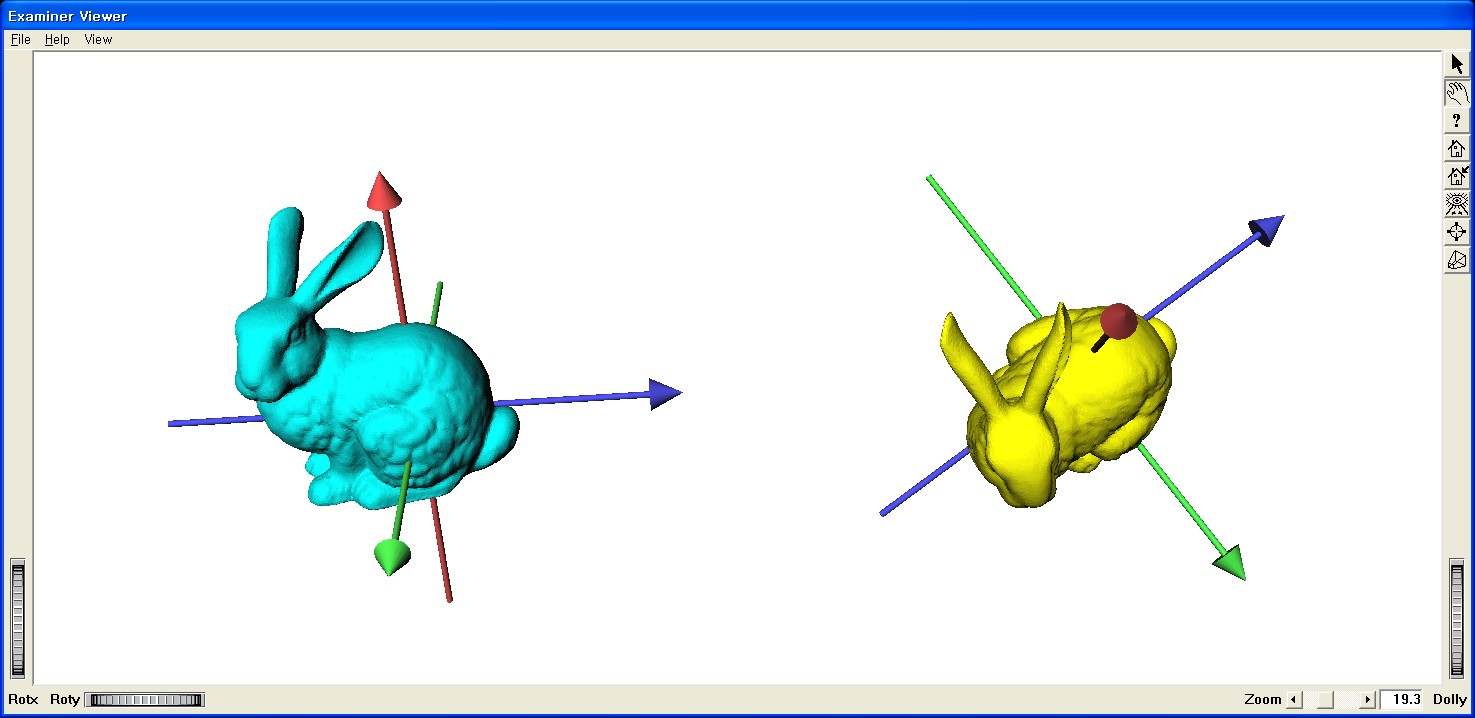
\includegraphics[width=0.45\textwidth]{bunny}
			\caption*{
				\textbf{point} : the 3d location of the bunny \\
				\textbf{vector} : translational movement\\
				\textbf{orientation}: the 3d orientation of the bunny\\
				\textbf{rotation} : circular movement
			}
		\end{SCfigure}
		
	\subsection{Teorema della rotazione di Eulero}
		The general displacement of a rigid body with
		one point fixed is a rotation about some axis.
		
		\noindent
		Qualsiasi rotazione si può esprimere come rotazione di un
		angolo rispetto a un asse.
		
		\noindent
		Qualsiasi rotazione lascia invariati un vettore invariato (l'asse).
		
		\noindent
		Una rotazione qualsiasi rispetto ad un asse passante per
		l'origine puo essere decomposta nel prodotto di tre rotazioni
		rispetto agli assi coordinati; i tre angoli prendono il nome di
		\textbf{angoli di Eulero}.
		
		\noindent
		La rappresentazione con gli angoli di Eulero non è univoca, a
		terne diverse può corrispondere la stessa trasformazione.\\
		Una delle rappresentazioni di Eulero impiega gli angoli roll (rollio),
		pitch (beccheggio) e yaw (imbardata), di derivazione aeronautica.
		
	\subsection{Problemi con angoli Eulero}
			Ci sono alcuni problemi con le rappresentazioni
			delle rotazioni
			\begin{itemize}
				\item Angoli di Eulero:
					Rotazioni non univoche:
					\[
						(z, x, y) [roll, yaw, pitch] = (90, 45, 45) = (45, 0, -45)
					\]
					mandano entrambi l'asse x in direzione $ (1, 1, 1) $
				\item Gimbal Lock (blocco del giroscopio)
				\begin{itemize}
					\item Gimbal è un dispositivo meccanico usato per
				supportare giroscopi o bussole
					\item Ci sono configurazioni problematiche
				\end{itemize}
				\item Interpolazione di rotazioni: Come calcoliamo il punto medio di una rotazione?
			\end{itemize}
	\subsection{Rotazione asse angolo}
		La rotazione generica asse angolo con asse r si può anche
		rappresentare con la seguente matrice, dove 
		$ c = \cos(\alpha) $ e $ s = \sin(\alpha) $:
		\[
			R(\alpha,\vec{r}) =
			\begin{pmatrix}
				(1-c)r^2_1 + c & (1-c)r_1 r_2 -s r_3 & (1-c) r_1 r_2 + s r_2 & 0 \\
				(1-c)r_1 r_2 + s r_3  & (1-c)r^2_2 +c & (1-c)r_2 r_2 -s r_1 & 0 \\
				(1-c)r_1 r_3 -sr_2 & (1-c) r_2 r_3 + s r_1 & (1-c)r^2_3 +c & 0 \\
				0 & 0 & 0 & 1 
			\end{pmatrix}
		\]
	\subsection{Matrici e proiezioni}
		\begin{enumerate}[label=\textbullet]
			\item Abbiamo il nostro mondo dove creare la scena inserendo i
		modelli: spazio Euclideo.
			\item Sappiamo trasformare i punti dello spazio traslando, ruotando
		e scalando.
			\item Per simulare la formazione delle immagini ci serve un ultimo
		strumento geometrico: la modellazione della proiezione degli
		oggetti sul piano immagine.
			\item Questo si fa con la proiezione prospettica o, in casi
		semplificati, con la proiezione ortografica o parallela
			\item Anche queste si possono modellare con matrici, solo che
		dovranno trasformare uno spazio 3D in uno 2D (espressi in
		coordinate omogenee). Quindi sono matrici.
		\end{enumerate}
	\subsection{La macchina fotografica virtuale}
		La metafora utilizzata per descrivere le relazioni
		scena/osservatore è quella della macchina fotografica virtuale
		(synthetic camera).\\
		Il modello semplice usato anche in Computer Vision è la
		\textbf{telecamera pinhole}.
		\begin{figure}[h!]
			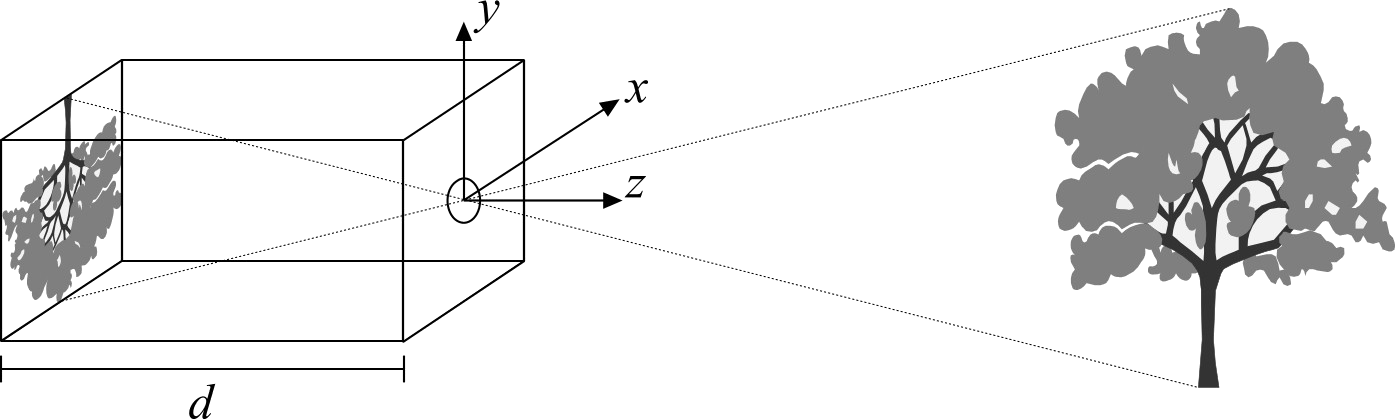
\includegraphics[width=0.5\textwidth]{virtual}
		\end{figure}
		
		La macchina fotografica	virtuale è costituita da un	parallelepipedo in cui la
		faccia anteriore presenta un foro di dimensioni	infinitesime (pinhole
		camera) e sulla faccia posteriore si formano le immagini.
		
		\vspace{-0.5cm}
		\begin{center}
			\begin{tikzpicture}[>=latex]
			\draw[->] (0,-1) -- (0,2) node[right] {$ \vec{y} $};
			\draw[densely dashed] (-3,0) -- (0,0);
			\draw[->] (0,0) -- (3.5,0) node[below] {$ \vec{z} $};
			\draw[densely dashed] (-3,-1) -- (3,1);
			\draw[densely dashed] (-3,1) -- (3,-1);
			\draw (-3,1) rectangle (0,-1);
			\draw[|<->|] (-3.2,1) -- (-3.2,-1) node[midway,left] {$ h $};
			\draw[|<->|] (-3,-1.2) -- (0,-1.2) node[midway,below] {$ d $};
			\draw[densely dashed, bend right] (2.1,-0.7) to (2.1,0.7); 
			\node[right] at (2.3,0.3) {$ \theta $};
			\end{tikzpicture}
		\end{center}
		
		Immagini nitide, nessun	problema di luminosità,	l’angolo di vista può essere modificato variando il rapporto tra la distanza focale (d) e la dimensione
		del piano immagine.\\
		Per convenzione (e maggiore semplicità) si assume l’esistenza
		di un piano immagine tra la scena ed il centro di proiezione \\
		Ne risulta il modello matematico della proiezione prospettica. \\
		
	\subsection{Proiezione prospettica}
		La relazione che lega i punti 3D ai punti sul piano in questa
		ipotesi è data dalla proiezione prospettica. Con semplici
		ragionamenti sui triangoli simili si ha che la proiezione di un
		punto $ P = (P_x, P_y, P_z) $ è data da:
		\begin{itemize}
			\item  $ P' = (-\dfrac{P_x d}{P_z}, -\dfrac{P_y d}{P_z}, 1) $ per il piano immagine dietro.
			\item $ P' = (\dfrac{P_x d}{P_z}, \dfrac{P_y d}{P_z}, 1) $, per il piano immagine davanti.
		\end{itemize}
		Possiamo scrivere la proiezione in forma matriciale:
		\[
			\vec{P'} =
			\begin{pmatrix}
				1 & 0 & 0 & 0 \\
				0 & 1 & 0 & 0 \\
				0 & 0 & 1/d & 1 
			\end{pmatrix}
			\begin{pmatrix}
				P_x \\
				P_y \\
				P_z \\
				1
			\end{pmatrix}
		\]
		
		Da un punto di vista geometrico, la proiezione è
		definita per mezzo di un insieme di rette di proiezione
		(i proiettori) aventi origine comune in un centro di
		proiezione, passanti per tutti i punti dell’oggetto da
		proiettare ed intersecanti un piano di proiezione.
		
		\noindent
		La proiezione di un segmento è a sua volta un
		segmento. Non è quindi necessario calcolare i proiettori di tutti i
		punti di una scena, ma solo quelli relativi ai vertici delle
		primitive che la descrivono.
		
		\noindent
		Le proiezioni geometriche piane si classificano in:
		\begin{itemize}
			\item Proiezioni \textbf{prospettiche} (distanza finita tra il centro ed il piano di
		proiezione)
			\item Proiezioni \textbf{parallele} (distanza infinita tra il centro ed il piano di
		proiezione)
		\end{itemize}
		\begin{figure}[h!]
			\centering
			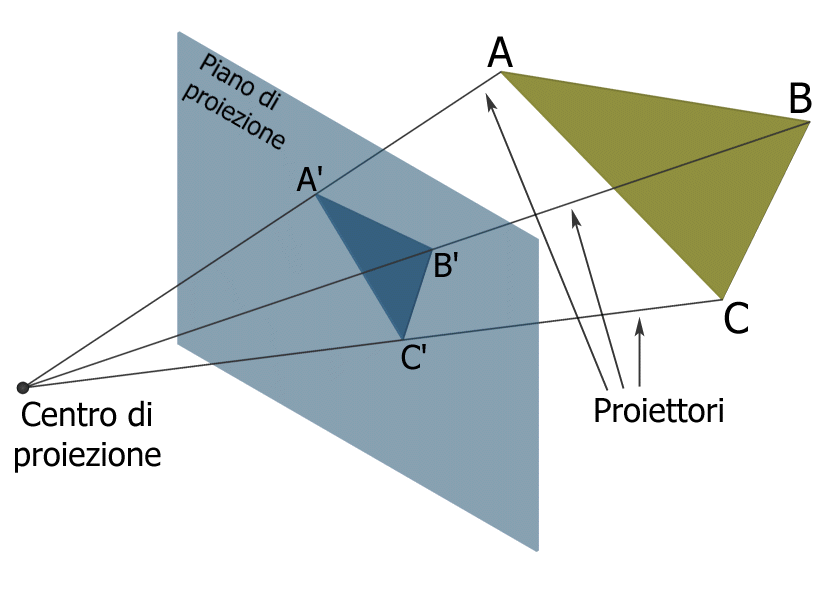
\includegraphics[width=0.4\textwidth]{proiez}
			\hspace{0.2cm}
			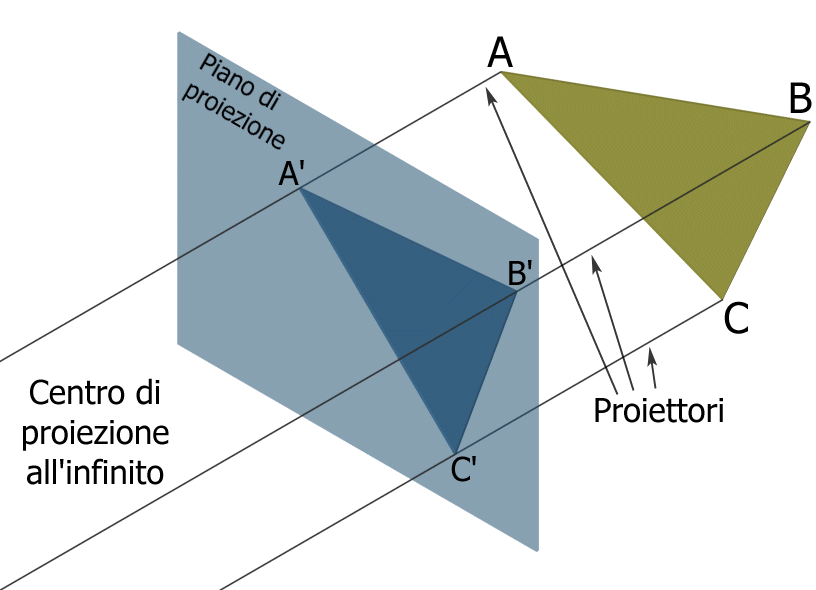
\includegraphics[width=0.4\textwidth]{proiez1}
		\end{figure}
		Al variare della distanza focale $ d $ si ha che:
		\begin{figure}[h!]
			\centering
			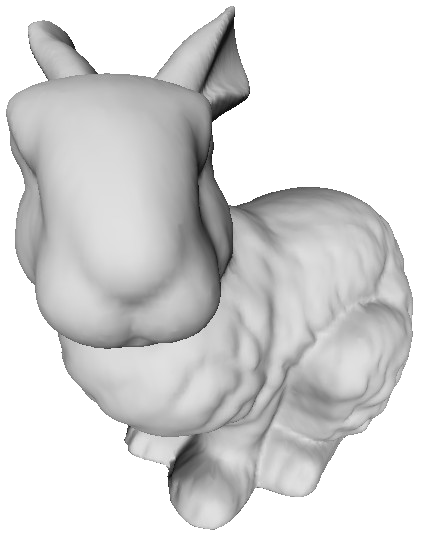
\includegraphics[width=0.13\textwidth]{proiez2}
			\hspace{0.2cm}
			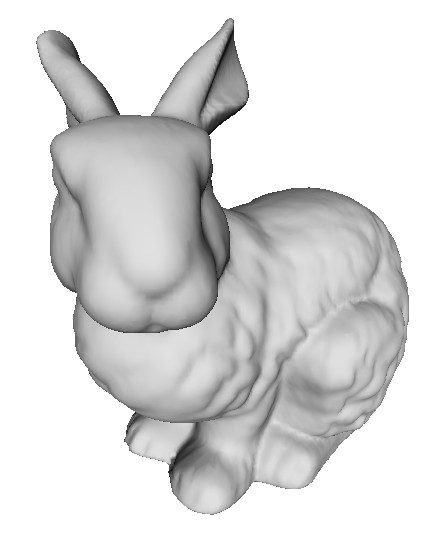
\includegraphics[width=0.15\textwidth]{proiez3}
			\hspace{0.2cm}
			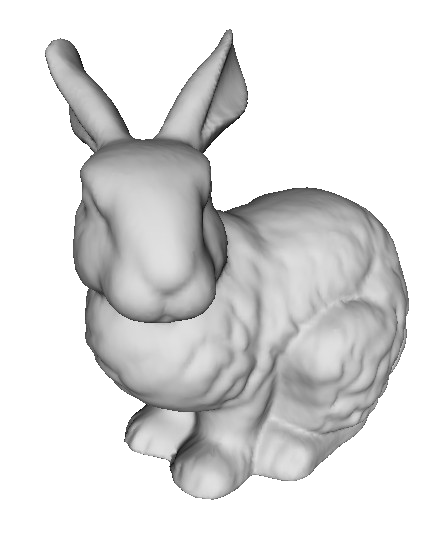
\includegraphics[width=0.15\textwidth]{proiez4}
			\hspace{0.2cm}
			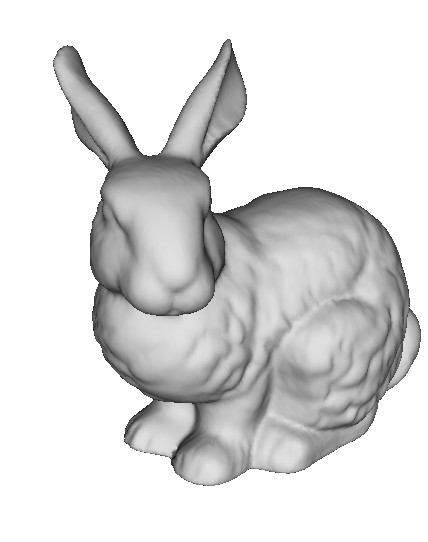
\includegraphics[width=0.15\textwidth]{proiez5}
			\hspace{0.2cm}
			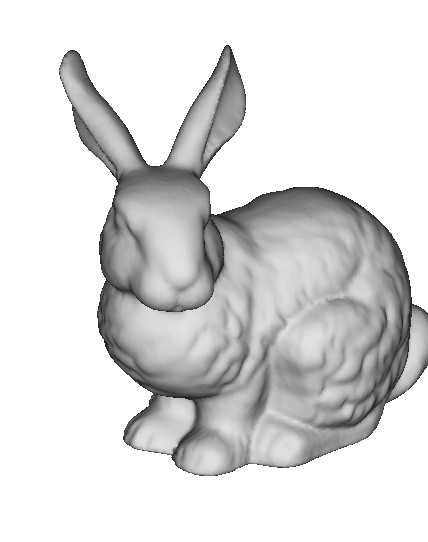
\includegraphics[width=0.15\textwidth]{proiez6}
			
			\begin{tikzpicture}
				\draw[red, thick] (-4,2.5) -- (-4,3) -- (-5,1) -- (-4,-1) -- (-4,-0.5);
				\node[box, draw=red, align = left, ] at (-2.5,1) {
					\footnotesize Più distorsione\\ \footnotesize prospettica\\
					\\
					\footnotesize Effetto "\textit{fish-eye}"\\\footnotesize  (grandangolo)};
				
				\node[box, draw=red, thick, align = left, ] at (2.5,1) {
					\footnotesize Proporzioni\\ \footnotesize più mantenute\\
					\\
					\footnotesize Effetto "\textit{zoom}"\\\footnotesize (es. vista
					dal satellite) };
				
				\draw[red, thick] (4,2.5) -- (4,3) -- (5,1) -- (4,-1) -- (4,-0.5);
				\node at (-5.25,3) {$ d $ piccolo};
				\node at (5.25,3) {$ d $ inifinito};
			\end{tikzpicture}
		\end{figure}
		
		\newpage
		Per motivi che capiremo, in grafica si usa in realtà
		rappresentare la proiezione prospettica con una
		trasformazione che mappa comunque sullo spazio 3D, quindi
		una matrice 4x4.
		
		\noindent
		Per passare alla rappresentazione 2D basta poi eliminare la z
		(che è sempre uguale a $ d $)
		\[
			\vec{P'} =
			\begin{pmatrix}
				1 & 0 & 0 & 0 \\
				0 & 1 & 0 & 0 \\
				0 & 0 & 1 & 0 \\
				0 & 0 & 1/d & 1
			\end{pmatrix}
			\begin{pmatrix}
				P_x \\
				P_y \\
				P_z \\
				1
			\end{pmatrix}
		\]
		In realtà la coordinata omogenea 2D che ricavo 
		dall'applicazione della matrice è 
		\[
			P' = (P_x, P_y ,P_z/d) 
		\]
		L'operazione che trasforma in 
		\[
			P' = (\dfrac{P_x d}{P_z}, \dfrac{P_y d}{P_z} ,1)	
		\]
		per avere la forma standard dei punti è la cosiddetta divisione.\\
		Prima della divisione i tre valori possono essere usati per
		rappresentare l'equivalenza dei diversi punti rispetto alla
		proiezione.
		
		\noindent
		Definiamo ora possibili strutture dati per modellare gli oggetti
		nello spazio.
		
		\noindent
		Poi vedremo come modellare anche la formazione delle
		immagini attraverso il "rendering".
		
\section{Modellare gli oggetti nello spazio}
	\begin{center}
		\begin{tikzpicture}[>=latex, scale=0.8,  every node/.style={scale=0.8}]
		\draw[dashed, rounded corners] (10,-4) rectangle (5,-0.5);
		\node[below] at (7.5, -4) {applicazione interattiva};
		\node[draw, rectangle, rounded corners, align=center] (a) {mondo reale,\\ modello matematico,\\ artista 3D ...};
		\node[draw, rectangle, fill=white, rounded corners, align=center, minimum height=1cm, minimum width=3cm] (b) at (4,-1.5) {Geometria};
		\node[draw, rectangle, rounded corners, align=center, minimum height=1cm, minimum width=3cm] (c)	at (8,-3) {Immagine/i};
		
		\draw[->, rounded corners] (a.east) -- ($ (a) + (4,0) $) node[right,align=left,yshift=0.5cm] {acquisizione 3D (scansione)\\simulazione (elementi finiti)\\modellazione (3DStudioMax, Maya)} -- (b.north);
		\draw[->, rounded corners] (b.south) -- ++(0,-1) -- ++(-3,0) node[below,align=left] {preprocessing\\(modelling)} -- ($ (b) + (-3,0) $) -- (b.west);
		\draw[->, rounded corners] (b.east) -- ($ (c) + (0,1.5) $) node[right] {rendering} -- (c.north);
		\end{tikzpicture}
	\end{center}
	
	\subsection{Geometria Analitica}
	Premessa: prima di vedere come si modellano gli oggetti,
	ricordiamo come si definiscono nello spazio Euclideo 3D le
	figure geometriche importanti dal punto di vista della
	modellazione grafica e del rendering.
	
	\noindent
	\textbf{Rette}: sono identificabili da un punto qualsiasi $ Q $ che giaccia sulla
	retta e da una direzione data da un versore $ u $. È facile vedere che
	sono il luogo dei punti dati da $ P = Q + t\vec{u} \quad t \in \R $\\
	In termini di componenti si vede facilmente che vale la seguente
	equazione 
	\[
		\dfrac{x - x_Q}{u_x} = \dfrac{y - y_Q}{u_y} = \dfrac{z - z_Q}{u_z}
	\]
	 
	Se si vuole specificare una retta dati due punti $ R $ e $ Q $, basta usare le
	formule date qui sopra tenendo conto che il versore che identica la
	retta e dato da: $ \vec{u}=\dfrac{(R-Q)}{|R-Q|} $
	
	\noindent
	\textbf{Semiretta}: basta aggiungere il vincolo $ t \geq 0 $
	
	\noindent
	\textbf{Segmenti}: dati i punti iniziale e finale $ P $ e $ Q $ possiamo scriverli come 
	$ P = Q + t(R-Q) \quad t \in \left[ 0; 1\right]  $
	
	\noindent
	\textbf{Sfere}: dato centro $ O $ e raggio $ r $, i punti della superficie sferica sono dati
	dall'equazione $ P = O + r\vec{u} $ con $ \vec{u} $ versore generico.
	Si dimostra facilmente che, in termini delle coordinate, la
	superficie sferica è data dall'equazione
	\[
		(x - x_0)^2 +(y - y_0)^2 +(z - z_0)^2 = r^2
	\]
	
	\noindent
	\textbf{Piani}: dati 3 punti non allineati $ P $, $ Q $ ed $ R $ il luogo dei punti che descrive
	il piano che li comprende è la combinazione affine
	\[
		S = \alpha P + \beta Q + \gamma R \quad \alpha,\beta, \gamma \in \R \quad \alpha+\beta+\gamma=1
	\]
	Alternativamente si puo definire un piano a partire da un punto $ Q $ che
	vi appartiene e da un vettore $ \vec{u} $ che ne identica la normale come il luogo
	dei punti $ P $ tali che $ (P - Q) \vec{u} = 0 $.
	In termini di coordinate abbiamo
	\[
		(x-x')u_x + (y-y')u_y + (z-z')u_z = 0
	\]
	Per passare dalla prima alla seconda rappresentazione basta
	prendere come punto $ Q $ e come vettore $ \vec{u} = (P-Q) \times (R-Q) $
	
	\noindent
	\textbf{Semispazi}: il piano di cui sopra identica due semispazi, uno
	positivo ed uno negativo:
	\begin{align*}
		(P-Q) \vec{u} &> 0 \\
		(P-Q) \vec{u} &< 0
	\end{align*}
	
	\subsection{Poligoni}
	
	\begin{wrapfloat}{figure}{I}{0pt}
		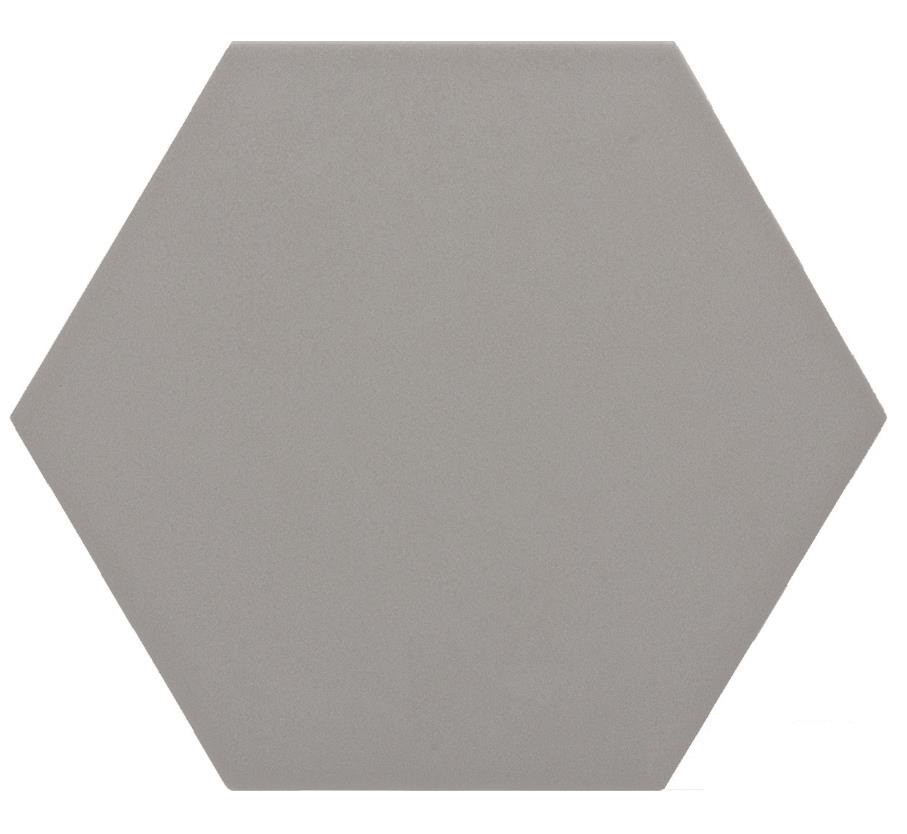
\includegraphics[width=0.2\textwidth]{poligono}
	\end{wrapfloat}
	
		Un poligono $ P $ è un insieme finito di segmenti (spigoli) di $ \R^2 $ , in
		cui ogni estremo (vertice) e comune a esattamente due
		segmenti, che si dicono adiacenti.\\
		Un poligono è detto semplice se ogni coppia di spigoli non
		adiacenti ha intersezione vuota.\\
		\textit{Teorema di Jordan}: Un poligono semplice $ P $ divide il piano in
		due regioni o facce, una limitata (detta interno di $ P $) ed una
		illimitata (detta esterno di $ P $).
		
		\noindent
		Per convenzione, un poligono viene rappresentato dalla
		sequenza dei suoi vertici $ P_1 \dots P_n $ ordinati in modo che l'interno
		del poligono giaccia alla sinistra della retta orientata da $ P_i $ a
		$ P_{i+1} $ , ovvero i vertici sono ordinati in senso antiorario.
		
		\begin{wrapfigure}{R}{0pt}
			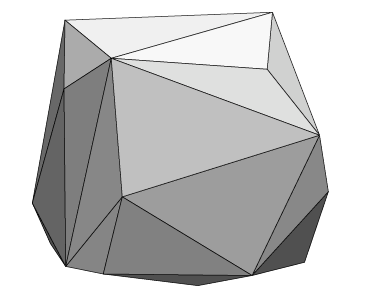
\includegraphics[width=0.2\textwidth, ]{poliedro}
		\end{wrapfigure}
		\noindent
	\subsection{Poliedri}
	
		In $ \R^3 $ un poliedro semplice e denito da un insieme finito di
		poligoni (facce) tali che ciascuno spigolo di una faccia e condiviso
		da esattamente un'altra faccia e le facce non si intersecano che
		negli spigoli.
		
	\subsection{Rappresentazione degli oggetti}
		Gli oggetti che si vogliono rappresentare in una applicazione
		grafica hanno di solito caratteristiche particolari
		\begin{itemize}
			\item Sono finiti
			\item Sono chiusi (non sempre)
			\item Sono continui
		\end{itemize}
		Le rappresentazioni di oggetti (regioni dello spazio, in
		generale) si suddividono in
		\begin{itemize}
			\item basate sul \textbf{contorno} (boundary): descrivono una regione in
		termini della superficie che a delimita (boundary representation, o
		b-rep).
			\item basate sullo \textbf{spazio occupato} (o volumetriche).
		\end{itemize}
		
		\newpage
		La rappresentazione più comune è quella di \textbf{maglie(mesh) di triangoli}:
		
		\begin{tikzpicture}[>=latex, scale=0.8,  every node/.style={scale=0.8}]
			\draw[->] (1,-1) -- (1,4) node [right] {x};
			\draw[->] (1,-1) --(4,-3) node [left] {z};
			\draw[->] (1,-1) -- (-5,-3) node [right] {y};
			\draw[ultra thick, fill=blue] (2.5,-1) -- (0,3) -- (-3,-1.5) -- cycle;
			\fill (0,3) circle (4pt) (a)
				(2.5,-1) circle (4pt) (b)
				(-3,-1.5) circle (4pt) (c);
			\node[yshift=0.2cm,above] at (0,3) {$v_0 = (x_0, y_0, z_0) $};
			\node[xshift=0.2cm,right] at (2.5,-1) {$v_1 = (x_1, y_1, z_1) $};
			\node[xshift=-0.2cm,left] at (-3,-1.5) {$v_2 = (x_2, y_2, z_2) $};
		\end{tikzpicture}
		
		\noindent
		Esistono però delle alternative:
		\begin{itemize}
			\item \textbf{Boundary}:
			Superfici parametriche (lisce, non hanno problemi di "tessellazione"
			cioè visibilità degli spigoli tra le facce)
			\item \textbf{Volumetriche}: 
			\begin{itemize}
				\item Rappresentazione "voxellizata" (a cubetti)
				\item Geometria costruttiva solida
			\end{itemize}
			\item \textbf{Image based rendering}:
			\begin{itemize}
				\item Non si modella effettivamente la scena, ma si memorizzano
				campionamenti della luce, renedendo però possibile una
				visualizzazione da più punti di vista, interattiva
				\item Light fields
			\end{itemize}
		\end{itemize}
		
		Il vantaggio principale nell’uso di superfici per modellare un
		oggetto sarebbe l’assenza del problema della tessellazione
		visibile (cioè approssimo una superficie lisca coi triangoli, ma
		vedo poi i triangoli evidenti, effetto ridotto di solito con
		trucchi opportuni nel rendering)\\
		L'uso di superfici parametriche risulta pesante per applicazioni in
		tempo reale; per lo più le superfici parametriche utilizzate in fase di modellazione o per
		rendering non interattivo.\\
		Negli ultimi tempi le cose sono cambiate ed oggi cominciano
		ad apparire applicazioni di grafica avanzata che usano superfici
		curve anche in tempo reale.
		
		Esempio: \textbf{curve/superfici di	Bezier}:
		Dati $ N $ punti di controllo la curva la curva passa per il
		primo e l'ultimo e approssima gli altri con una funzione da
		essi dipendente. Con una griglia si generano superfici.
		
		\begin{figure}[h!]
			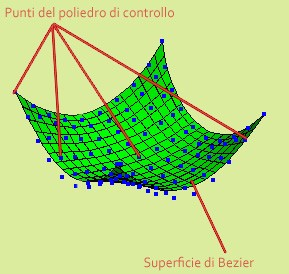
\includegraphics[scale=0.5]{superf}
			\hspace{0.2cm}
			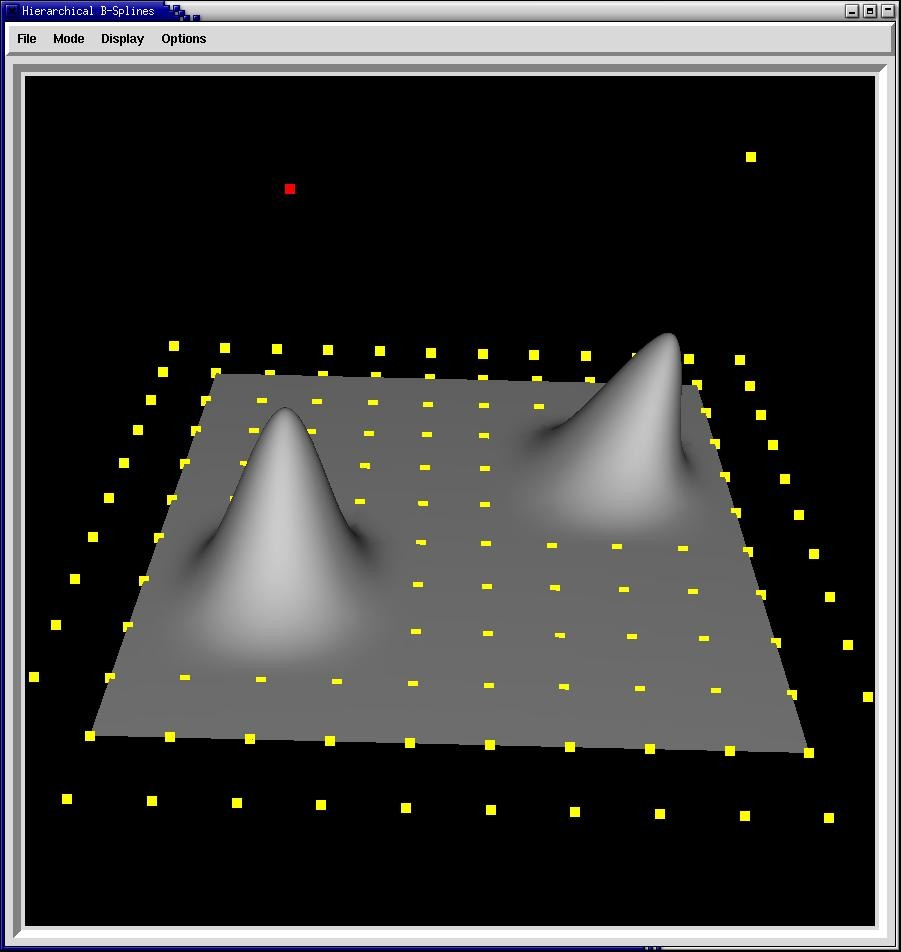
\includegraphics[scale=0.15]{superf1}
			\hspace{0.2cm}
			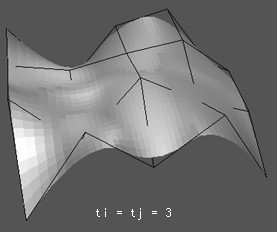
\includegraphics[scale=0.4]{superf2}
		\end{figure}
		
		\subsubsection{Geometria costruttiva solida (CSG)}
		
		Altra rappresentazione particolarmente adatta per il modeling
		(diffusa nel settore CAD), ma poco efficiente per il rendering è quella della
		\textbf{Geometria costruttiva solida (CSG)}.\\
		Si tratta, essenzialmente, di costruire degli oggetti geometrici
		complessi a partire da modelli base con operazioni booleane
		
		\noindent
		\textbf{Operazioni:}
		\begin{itemize}
			\item \textbf{Unione}: l’unione $ A \cup B $ è l’insieme dei punti che appartengono
			ad almeno uno dei due solidi (or non esclusivo).
			\item \textbf{Differenza}: la differenza $ A \setminus B $ è l’insieme dei punti che
			appartengono ad $ A $, ma non a $ B $.
			\item \textbf{Intersezione}: l’intersezione $ A \cap B $ è l’insieme dei punti che
			appartengono ad $ A $ ed a $ B $ (and).
			\item Le operazioni CSG possono essere descritte tramite un albero
			(gerarchia).
			Ciascun nodo di un albero che non sia una foglia contiene una
			delle tre operazioni elementari $ \cup $ , $ \cap $ o $ \setminus $.
			Ciascuna foglia contiene una primitiva.
		\end{itemize}
		
		\subsubsection{Acquisizione dal vero: point clouds}
			Un modo per generare modelli 3D per mondi virtuali è
			acquisire dal vero.\\
			La scansione 3D, oggi tecnologia matura con diverse tecnologie
			Laser, luce strutturata, visione computazionale.\\
			Gli scanner (esattamente come le macchine fotografiche in 2D)
			di fatto non acquisiscono un modello del mondo, ma
			campionano la geometria (con eventuali attributi, es. colore) in
			una serie di punti discreti: si parla di \textbf{nuvole di punti (point
			clouds)}
		
		\subsubsection{Partizionamento spaziale (voxel)}
			Lo spazio viene suddiviso in celle adiacenti dette in 3D voxel
			(equivalente dei pixel delle immagini): una cella è "piena" se
			ha intersezione non vuota con la regione, è detta vuota in
			caso contrario. Oppure contiene un valore di densità (tipico
			dei dati diagnostici es. TAC)\\
			Una rappresentazione di una scena complessa ad alta
			risoluzione richiederebbe l’impiego di un numero enorme
			numero di voxel, per cui questa rappresentazione è in genere
			limitata a singoli oggetti.\\
			Ma le cose stanno cambiando grazie a
			progressi nell'HW e nel SW.\\
			Rendering di modelli voxel-based:
			\begin{itemize}
				\item Algoritmi ad hoc (tecniche direct volume rendering)
				\item conversione da voxel a rappresentazione per superfici (triangle-
				based)
			\end{itemize}
			Da una rappresentazione volumetrica voxelizzata si può
			passare efficientemente a una rappresentazione poligonale
			della superficie mediante l’algoritmo detto marching cubes.
		
		\subsubsection{Rappresentazioni compatte(Octree)}
			Se ho solo i valori pieno/vuoto, posso rappresentare in modo
			compatto il volume con una struttura \textbf{octree}.\\
			Si parte con un cubo contenente la regione e si suddivide
			ricorsivamente. Ci si ferma ogni volta che un ottante contiene
			tutte celle piene o tutte celle vuote.\\
			Più economica rispetto alla enumerazione delle singole celle,
			poiché grandi aree uniformi (piene o vuote) vengono
			rappresentate con una sola foglia (anche se nel caso peggiore
			il numero delle foglie è pari a quello delle celle).

			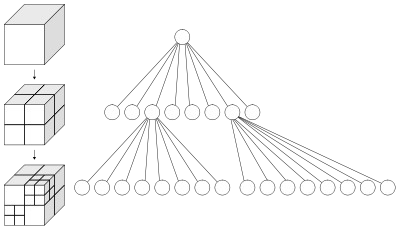
\includegraphics[scale=0.4]{octree}
			\hspace{2.5cm}
			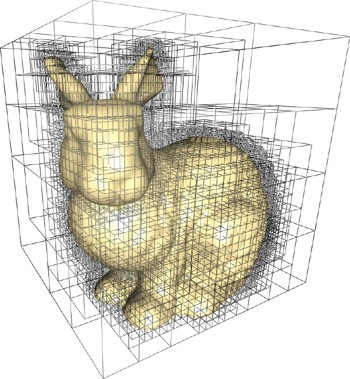
\includegraphics[scale=0.3]{octree2}
			
			Le strutture di partizionamento spaziale sono anche utili per
			"contenere" le geometrie poligonali: come vedremo consente
			di rendere più semplice la ricerca di intersezioni tra oggetti e
			con i raggi ottici.
			
	\subsection{Maglie poligonali (mesh)}
		Nella grafica 3D interattiva si usa quasi sempre la modellazione
		basata su approssimazione poligonale degli oggetti (del loro
		contorno: è una \textit{boundary representation}).\\
		Si tratta di approssimare una superficie 2D con un insieme di
		poligoni convessi opportunamente connessi gli uni agli altri.\\
		Nella pipeline di rendering si lavora in genere con i soli
		\textbf{triangoli}:
		tutte le altre rappresentazioni eventualmente usate nel programma
		sono convertite prima del rendering in triangoli
		Possiamo usare la geometria per definire rigorosamente le
		proprietà dei modelli triangolati.
		
		\bigskip
		\noindent
		Una \textbf{varietà} $k$-dimensionale $ X $ è un sottoinsieme di $ \R^d$  in cui
		ogni punto ha un intorno omeomorfo alla sfera aperta di $ \R^k $.\\
		In generale le superifici degli oggetti solidi (sfere, poliedri, ecc.)
		sono varietà bidimensionali.\\
		\textbf{Omeomorfismo}: applicazione biiettiva, continua, con inversa
		continua. Intuizione: trasformazione senza "strappi".
		In una varietà $k$-dimensionale con bordo ogni punto ha un intorno
		omeomorfo alla sfera aperta o alla semisfera aperta di $ \R^k $ .\\
		Il bordo di $ X $ è l’insieme dei punti che hanno un intorno omeomorfo
		alla semisfera aperta.
		Una varietà è sempre una varietà con bordo, eventualmente vuoto.\\
		Il bordo, se non è vuoto, è a sua volta una varietà $ k-1 $ dimensionale
		senza bordo.
		
		\bigskip
		Una \textbf{maglia (mesh) triangolare} è un'insieme di triangoli le cui
		intersezioni siano esclusivamente vertici e lati (spigoli) dei
		triangoli e che sia anche una varietà bidimensionale con bordo.
		Due triangoli che condividono un lato si dicono adiacenti
		I triangoli della maglia si chiamano anche facce.\\
		La condizione di essere varietà si traduce nei seguenti vincoli
		sulla struttura:
		\begin{itemize}
			\item uno spigolo appartiene al massimo a due triangoli (quelli eventuali
			che appartengono ad uno solo formano il bordo della maglia)
			\item se due triangoli incidono sullo stesso vertice allora devono essere
			raggiungibili l'uno dall'altro attraverso un percorso tra triangoli
			adiacenti ovvero devono formare un ventaglio o un ombrello.
		\end{itemize}
		Si usa il termine condizione 2-manifold (varietà)
		
		\begin{tikzpicture}[ scale=0.3,  every node/.style={scale=0.3}]
			\draw[fill=OliveGreen!90!] (1,0) -- (4.5,-5) -- (5,6) -- cycle;
			\draw[fill=gray!70!] (12,-1) -- (5,6) -- (-5,-3) -- (1,0) -- cycle;
			\draw (1,0) -- (5,6);
			\draw[densely dashed] (4.5,-5) -- (5,6);
			\fill (5,6) circle (10pt) (a)
				(1,0) circle (10pt) (b);
			\draw[ultra thick, red] (5,6) -- (1,0);
			\node[right, xshift=1cm, text =red] at (5,6) {\Huge \textbf{NO}};
		\end{tikzpicture}
		\hspace{2.5cm}
		\begin{tikzpicture}[ scale=0.3,  every node/.style={scale=0.3}]
		\draw[fill=OliveGreen!90!] (1,0) -- (4.5,-5) -- (5,6) -- cycle;
		\draw[fill=gray!70!] (12,-1) -- (5,6) -- (1,0) -- cycle;
		\draw (1,0) -- (5,6);
		\draw[densely dashed] (4.5,-5) -- (5,6);
		\fill (5,6) circle (10pt) (a)
		(1,0) circle (10pt) (b);
		\draw[ultra thick, Green] (5,6) -- (1,0);
		\node[right, xshift=1cm, text =Green] at (5,6) {\Huge \textbf{SI}};
		\end{tikzpicture}
		
		\begin{tikzpicture}[ scale=0.3,  every node/.style={scale=0.3}]
			\draw[fill=TealBlue!30!] (-5,-3) -- (1,0) -- (5,6) -- cycle;
			\draw[fill=TealBlue!30!] (4,0) -- (9,-1) -- (5,6.2) -- cycle;
			\draw[fill=TealBlue!30!] (10,-1.5) -- (5.2,6.3) -- (13,7) -- cycle;
			\node[above, yshift=1cm, text =red] at (5,6) {\Huge \textbf{NO}};
		\end{tikzpicture}
		\hspace{2.5cm}
		\begin{tikzpicture}[ scale=0.3,  every node/.style={scale=0.3}]
			\draw[fill=TealBlue!30!] (-5,-3) -- (1,0) -- (5,6) -- cycle;
			\draw[fill=CornflowerBlue] (1,0) -- (10,-1.5) -- (5,6) -- cycle;
			\draw[fill=TealBlue!30!] (10,-1.5) -- (5,6) -- (13,7) -- cycle;
			\node[above, yshift=1cm, text =Green] at (5,6) {\Huge \textbf{SI}};
		\end{tikzpicture}
		
		Il bordo della maglia consiste di uno o	più anelli (sequenza chiusa di spigoli) o
		loop.\\
		Se non esistono spigoli di bordo la	maglia è chiusa (come quelle che
		rappresentano la superficie di una sfera).\\
		L’\textbf{orientazione} di una faccia è data dall’ordine ciclico (orario o antiorario)
		dei suoi vertici incidenti. L’orientazione determina il fronte ed il retro della
		faccia. La convenzione (usata anche da OpenGL) è che la faccia mostra il fronte.
		
		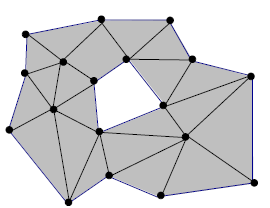
\includegraphics[scale=0.5]{orient}
		\hspace{2.5cm}
		\begin{tikzpicture}[scale=0.5]
			\node[above] at (-3,4) {Fronte};
			\node[above] at (3,4) {Retro};
			\draw[fill=Gray!80!] (-1,0) -- (-3,3) -- (-4,-2) -- cycle;
			\draw (1,0) -- (3,3) -- (4,-2) -- cycle;
			\fill (-1,0) circle (5pt) coordinate [label=below:$V_2$]  (a) 
				(-3,3) circle (5pt) coordinate [label=above:$V_3$] (b)
				(-4,-2) circle (5pt) coordinate [label=below:$V_1$] (c)
				(1,0) circle (5pt) coordinate [label=below:$V_2$] (d)
				(3,3) circle (5pt) coordinate [label=above:$V_3$] (d)
				(4,-2) circle (5pt) coordinate [label=below:$V_1$] (d);
		\end{tikzpicture}
		
		\noindent
		L’orientazione di due facce adiacenti è compatibile se i due
		vertici del loro spigolo in comune sono in ordine inverso. Vuol
		dire che l’orientazione non cambia attraversando lo spigolo in
		comune.\\
		La maglia si dice \textbf{orientabile} se esiste una scelta
		dell’orientazione delle facce che rende compatibili tutte le
		coppie di facce adiacenti.
		
			\begin{figure}[h!]
				\centering
				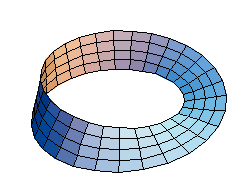
\includegraphics[scale=0.5]{moebius}
				\caption{Non tutte le mesh 2-manifold sono
					orientabili (es. anello di Moebius)} 
			\end{figure}
		
		Abbiamo definito la maglia triangolare. In maniera analoga si
		può estendere la definizione a maglie poligonali generiche\\
		\textbf{Maglie poligonali generiche}: i poligoni possono avere qualsiasi
		numero di spigoli e non è detto che ci sia un solo tipo di poligono.
		Sono raramente utilizzate in grafica al calcolatore\\
		\textbf{Quadrangolari} (quad meshes): gli elementi poligonali sono tutti
		quadrilateri. Sono alle volte usate, per esempio se si vuole fare il
		rendering di un terreno descritto da un array di altezze.\\ In una
		maglia quadrangolare bisogna imporre un vincolo aggiuntivo di
		planarità per ogni quadrilatero che la compone.\\
		OpenGL consente di descrivere maglie poligonali generiche, ma
		per disegnarle li suddivide usualmente in triangoli.
		
	\subsubsection{Equazione di Eulero}
		Se $ V $ è il numero di vertici, $ L $ il numero di spigoli ed $ F $ il numero di
		facce della maglia poligonale orientabile chiusa di genere G, allora
		vale la Formula di Eulero $ V - L + F = 2 - 2G $
		Una superficie ha genere $ G $ se può essere tagliata lungo $ G $
		linee semplici chiuse senza disconnetterla (intuitivamente,
		ma non rigorosamente “numero di buchi”).\\
		l genere di una superficie determina la sua
		topologia; per una sfera, per esempio, $ G = 0 $,
		mentre per un toro (una ciambella) $ G = 1 $.\\
		Più in generale, per una maglia poligonale orientabile (e varietà
		bidimensionale) vale la formula $ V - L + F = 2(S - G) - B $\\
		$ S $ numero di componenti connesse, $ B $ è il numero di anelli di bordo.
		
	\subsection{Mesh di triangoli}
		Nella pratica sono il tipo di modello dominante, usato nella gran parte delle applicazioni interattive dato che il rendering è ottimizzato in hardware.\\
		Generate da modellazione CAD, acquisizione con scanner,
		ricostruzione da immagini (Computer Vision).\\
		Il numero di poligoni determina il dettaglio, ma il costo in
		memoria può essere notevole.
		
	\subsection{Costruzione della mesh triangolare}
		Conversione da altri formati:
		\begin{itemize}
			\item Poligoni $ \longrightarrow $ Triangoli
			\item Superf. Quadriche $ \longrightarrow $ Triangoli
			\item Campi di altezze o Punti $ \longrightarrow $ Triangoli
		\end{itemize}
		Per rappresentare gli oggetti con le proprietà fisiche relativa a
		colore e riflessione della luce, devo abbinare alla geometria dei
		valori di proprietà (\textit{attributi})\\
		Posso definirli:
		\begin{itemize}
			\item per vertice: esplicito un attributo per ogni vertice
			\item per faccia: esplicito un attributo per ogni faccia
			\item per wedge (vertice di faccia): esplicito tre attributi per ogni faccia
		\end{itemize}
		Attributi più comuni: Colore, Normali (versori perpendicolari), coordinate texture.\\
		Non è sempre semplice modellare le entità da rappresentare
		con triangoli. Ad esempio: Nuvole, Fiamme, Capelli, pelliccia etc.
		
		\bigskip
		
		Quando si devono disegnare due triangoli con uno spigolo in
		comune, questo viene disegnato due volte. Questo introduce
		un certo grado di ridondanza che può incidere sulle prestazioni.\\
		Si preferisce quindi raggruppare i triangoli di una maglia in
		opportuni gruppi che possono essere elaborati in maniere più
		efficiente. Si possono ad esempio utilizzare:
		\begin{itemize}
			\item \textbf{Fan di triangoli}: è un gruppo di triangoli che hanno in comune un
			vertice. Il primo viene specificato completamente, per i successivi
			basta dare il nuovo vertice. Efficiente, ma i triangoli che incidono su
			un vertice sono in genere pochi.
			\item \textbf{Strip di triangoli}: gruppo di triangoli che posseggono a due a due
			uno spigolo in comune. Di nuovo il primo triangolo viene specificato
			normalmente, per i successivi basta specificare il nuovo vertice.
			Meno efficiente, ma le strip in genere contengono più triangoli delle
			fan.
		\end{itemize}
		Esistono algoritmi per creare queste rappresentazioni dalle
		mesh.
		
	\subsection{Mesh e rendering}
		Per determinare l’effetto di una qualsiasi trasformazione affine
		su un oggetto (traslazione, rotazione, scalatura, composizioni
		varie di queste), basta applicare la trasformazione ai vertici
		(che sono punti); le informazioni connettive date dagli spigoli
		non cambiano in questo tipo di trasformazioni.\\
		Questo rende piuttosto semplice il rendering di oggetti descritti in
		termini di maglie poligonali. Qualsiasi trasformazione viene eseguita
		sui vertici, cioè si tratta di applicare trasformazioni affini su punti.\\
		L’affermazione precedente è vera anche per la proiezione; per vedere
		come si proietta la forma di una maglia su un piano (l’immagine),
		basta seguire la proiezione dei vertici.
		
	\subsection{Memorizzazione}
		Alla creazione dei modelli vengono in genere generati nodi,
		connettività e attributi. Gli algoritmi di processing e rendering
		devono accedere in vario modo a tale informazione.
		Esistono diversi modi di rappresentare questa informazione.\\
		Nei programmi applicativi sono quindi necessarie delle
		procedure per convertire una rappresentazione in un’altra. \\
		Progettare ed implementare tali procedure è un ottimo modo
		per capire nel dettaglio le varie rappresentazioni utilizzate per
		descrivere maglie poligonali.\\
		Nei disegni e negli esempi ci concentreremo sul caso di maglia
		triangolare, ma il discorso è valido in generale per tutti i
		poligoni convessi.
	\subsection{Elementi base}
		\textbf{Vertici}: sono gli elementi 0 dimensionali e sono identificabili
		con punti nello spazio 3D (essenzialmente tre coordinate);
		alle volte può essere utile associare ai vertici altre
		caratteristiche oltre alla posizione (tipo il colore).\\
		\textbf{Spigoli}: sono elementi 1 dimensionali e rappresentano un
		segmento che unisce due vertici. Di solito non contengono
		altre informazioni.\\
		\textbf{Facce}: sono i poligoni bidimensionali, formati da un certo
		numero di spigoli e di vertici (dimostrare che sono in numero
		uguale). I vertici o gli spigoli si usano per identificare la faccia;
		possono contenere altre informazioni (tipo il colore).\\
		\textbf{Normali}: è fondamentale sapere quale è l’esterno della
		superficie e quale l’interno, e qual è l'orientazione locale della
		superficie; a tal scopo si associa spesso ad una maglia
		poligonale anche l’informazione sulla normale uscente.\\
		La normale $ \vec{n} $ ad una faccia è data dal prodotto vettore di due
		suoi spigoli consecutivi non collineari:\\
		Attenzione al verso: la normale è uscente dal fronte della faccia\\
		Per un triangolo $ (V_1 ,V_2 ,V_3 ) $ si ha: $ \vec{n} = (V_3 -V_2)\times(V_1 -V_2 ) $.
		
		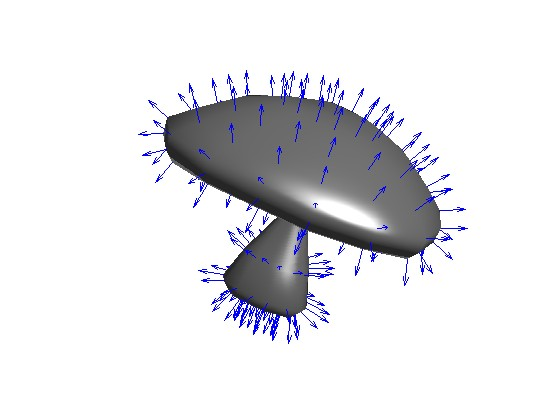
\includegraphics[scale=0.3]{norm}
		
		Attenzione (vedremo in lab): ci servono le normali per
		calcolare il modello di Phong. Le possiamo calcolare per i
		modelli, cui poi sono applicate le trasformazioni geometriche e
		di proiezione.\\
		Ma se applichiamo trasformazioni generiche ai modelli queste
		trasformazioni non preservano necessariamente l'ortogonalità
		di normale e superficie.\\
		Per trasformare senza questo problema le normali possiamo
		trasformarle con una matrice diversa.\\
		Consideriamo un vettore tangente $ \vec{t} $ alla superficie:
		\begin{align*}
			\vec{n}\vec{t}^T &= 0 \\
			\vec{n} M^{-1} M\vec{t} &= 0 \\
			(M^{-1})^T \vec{n} M\vec{t} &= 0
		\end{align*}
		
		Quindi la normale trasformato da $ (M^{-1})^T\vec{n} $ è perpendicolare alla
		superficie trasformata. Cioè per evitare problemi si
		trasformeranno le normali con l'inversa trasposta della matrice
		di trasformazione del modello.
		
	\subsection{Struttura della mesh}
		I vertici danno informazioni di tipo posizionale, gli spigoli
		informazioni di tipo connettivo (non c'è informazione spaziale).\\
		Gli spigoli connettono i vertici, permettendo di introdurre un
		concetto di “vicinanza” tra vertici e dando le informazioni di
		tipo topologico (ovvero definiscono un grafo).\\
		Le facce sono determinate una volta dati i vertici e gli spigoli,
		quindi non introducono nulla.\\
		Al più possono avere associati attributi, anche se è raro.\\
		
		\bigskip
		
		Ci sono vari modi di conservare le informazioni sui modelli.
		Questi possono differire per
		\begin{itemize}
			\item Memoria occupata
			\item Complessità di implementazione di operazioni di ricerca (es. ricerche
			di adiacenza
			\begin{itemize}
				\item Quali sono i vertici vicini a uno dato?
				\item Quali sono gli spigoli che contengono un vertice dato?
				\item Quali sono le facce che contengono uno spigolo?
				\item ...
			\end{itemize}
		\end{itemize}
		Possibilità di controllo sulla qualità delle superfici (es. manifoldness)
		
	\subsection{Lista di triangoli e indexed}
		\begin{itemize}
			\item Immediata: specificare tutte le facce della maglia come
			terne di triplette di coordinate cartesiane
			\item Spreco di memoria: duplico le coordinate. Meglio usare
			una struttura indicizzata, con la lista dei vertici e la
			lista delle facce con i	puntatori ai vertici (indici)
			\item Normalmente usate in openGL per il rendering
			\item Non ottimali per le ricerche
		\end{itemize}
		\begin{multicols}{2}
			\begin{lstlisting}
typedef struct{
	float v1[3];
	float v2[3];
	float v3[3];
} faccia;
			\end{lstlisting}
			\columnbreak
		\begin{lstlisting}
typedef struct {
	float x,y,z;
} vertice;
typedef struct {
	vertice* v1,v2,v3;
} faccia;
		\end{lstlisting}
		\end{multicols}
		
		\begin{figure}[h!]
			\vspace*{-1.2cm}
			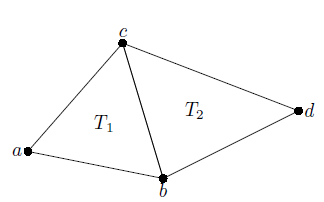
\includegraphics[scale=0.4]{mesh}
		\end{figure}
	
	\subsection{Winged edge (Baugmart 1975)}
		Si aggiungono dei puntatori allo spigolo per
		rendere più semplice l’analisi delle incidenze.\\
		L’elemento base è lo spigolo (edge) con le sue due facce incidenti (wings):
		\begin{itemize}
			\item Lo spigolo $ l_2 $ contiene un puntatore ai due
			vertici su cui incide (b; c), alle due facce su cui
			incide $ (T_1, T_2) $ ed ai due spigoli uscenti da
			ciascun vertice
			\item Un vertice contiene un puntatore ad uno degli
			spigoli che incide su di esso, più le coordinate
			(ed altro)
			\item La faccia contiene un puntatore ad uno degli
			spigoli che vi incide (ed altro).
		\end{itemize}
		La struttura assume che ogni spigolo non di
		bordo abbia due facce incidenti (manifold).
		
		\begin{multicols}{2}
		\begin{lstlisting}
typedef	struct{
	we_vertice* v_ini, v_fin;
	we_spigolo* vi_sin, vi_dstr;
	we_spigolo* vf_sin, vf_dstr;
	we_faccia* f_sin, f_dstr;
} we_spigolo;
typedef struct {
float x, y, z;
	we_spigolo* spigolo;
} we_vertice;
typedef struct {
	we_spigolo* spigolo;
} we_faccia;
		\end{lstlisting}
		
		\columnbreak
		
		\vspace*{1cm}
			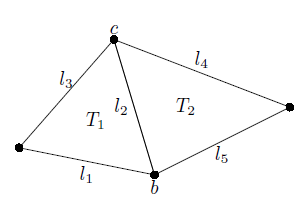
\includegraphics[scale=0.5]{mesh1}
		\end{multicols}
		
	\subsection{Half edge}
		Ogni spigolo viene diviso in due spigoli
		orientati in modo opposto:
		\begin{itemize}
			\item Ciascun mezzo spigolo contiene un puntatore
			al vertice iniziale, alla faccia a cui “appartiene”,
			al mezzo spigolo successivo (seguendo
			l’ordinamento) ed al mezzo spigolo gemello
			\item Ogni vertice, oltre alle coordinate (e attributi)
			contiene un puntatore ad uno qualsiasi dei
			mezzi spigoli che esce da tale vertice
			\item Ogni faccia contiene uno dei suoi mezzi spigoli
			(oltre ad altre caratteristiche quali, ad
			esempio, la normale)
		\end{itemize}
		Efficiente per le ricerche ed elegante.
		
		\begin{multicols}{2}		
	\begin{lstlisting}
typedef struct {
	he_vertice* origine;
	he_spigolo* gemello;
	he_faccia* faccia;
	he_spigolo* successivo;
} he_spigolo;
typedef struct {
	float x, y, z;
	he_spigolo* spigolo;
} he_vertice;
typedef struct {
	he_spigolo* spigolo;
} he_faccia;
	\end{lstlisting}
		
		\columnbreak
		
		\vspace*{1cm}
		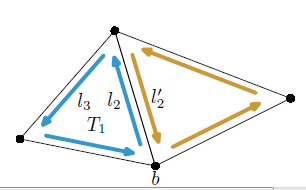
\includegraphics[scale=0.5]{mesh2}
	\end{multicols}
		
	\noindent
	\textbf{Note:}\\
	La stessa applicazione grafica può far uso di più di una
	struttura dati.\\
	La rappresentazione con la lista di vertici essendo semplice e
	leggera è tipicamente usata come formato per i file
	contenenti la geometria di oggetti.\\
	Le applicazioni grafiche in genere caricano tali file ed usano
	l’informazione contenuta in essi per riempire una struttura
	dati più utile ai fini algoritmici (per esempio la half-edge).
	
	
	\section{Rendering}
\end{document}	